\documentclass[a4paper]{report}
\usepackage[utf8]{inputenc}
\usepackage[T1]{fontenc}
\usepackage{RJournal}
\usepackage{amsmath,amssymb,array}
\usepackage{booktabs}
\usepackage{subcaption}
\usepackage{tikz}  
\usetikzlibrary{shapes.geometric, arrows.meta, positioning}

% DO NOT define your own macros.
% This just makes it harder to create the html version of your article for the website.

\begin{document}

%% do not edit, for illustration only
\sectionhead{Contributed research article}
\volume{18}
\volnumber{3}
\year{2026}
\month{September}
\setcounter{page}{1}

%% replace RJtemplate with your article
\begin{article}
  % !TeX root = RJwrapper.tex
\title{R Package dbrobust: Robust Distance-Based Visualization and Analysis of Mixed-Type Data}
\author{by Eva Boj, Aurea Grané and Marcos \'Alvarez}

\maketitle

\begin{abstract}
In many applied fields, such as socioeconomic research, quality of life analysis or gender inequality studies, datasets often contain a mixture of quantitative, binary and categorical variables. Traditional multivariate techniques face this complexity, especially when robustness to outliers and interpretability in high-dimensional spaces is required. To overcome these challenges and address the lack of integrated tools for robust distance-based (DB) analysis of mixed-type data, we introduce \CRANpkg{dbrobust}, a new R package that provides a unified and extensible framework for computing, visualizing and analyzing robust distances between observations. The package builds on classical measures such as Euclidean, Manhattan, Mahalanobis and Gower distances, and extends them through robust and weighted generalizations, including a novel implementation of a family of hybrid distances via Related Metric Scaling (RelMS). It integrates visualization techniques such as distance heatmaps, graph-based layouts and multidimensional scaling (MDS) maps, including conditional MDS to highlight trimmed individuals or reveal structural patterns across groups, and is fully compatible with \CRANpkg{dbstats}, which implements the distance-based predictive models.
\end{abstract}

\section{Introduction}
\label{sec.introduction}

Contemporary applied statistics faces growing complexity in domains such as social sciences, quality of life assessment, environmental monitoring, and gender inequality research. Analysts increasingly encounter datasets of mixed-type that combine quantitative, binary, and multiclass categorical variables, reflecting multifaceted phenomena in the real world. Traditional statistical models frequently rely on assumptions of distributional homogeneity and well-behaved data structures that rarely hold in practice. These limitations are compounded by challenges including influential outliers, measurement inconsistencies, and the curse of dimensionality, which collectively undermine the efficacy of classical approaches in extracting meaningful insights from complex datasets.

The analysis of mixed-type variables presents substantial methodological hurdles. Conventional multivariate techniques, such as principal components analysis and multivariate analysis of variance, are fundamentally designed for continuous data and often yield biased or uninterpretable results when applied to categorical or binary variables. Their sensitivity to anomalous observations further distorts both parametric estimation and graphical representations. Perhaps most critically, the absence of a standardized framework for quantifying dissimilarity across diverse variable types creates significant obstacles for both exploratory data examination and confirmatory statistical inference, necessitating specialized methodological approaches.

DB methodologies offer a promising alternative by reducing multivariate complexity to pairwise dissimilarity computations. While established measures exist for homogeneous data (e.g., Euclidean and Mahalanobis distances for continuous variables; Jaccard and Sokal similarity coefficients for binary data), the Gower similarity coefficient provides a unified approach for mixed-type variables. However, conventional distance measures often lack robustness against data contamination. Recent advances have introduced more robust and adaptive formulations, but their implementation remains fragmented across statistical ecosystems, limiting accessibility for applied researchers.

This work addresses these challenges through the development and comprehensive documentation of \CRANpkg{dbrobust} \citep{dbrobust}, a novel R package \citep{R} designed for robust DB analysis. It pursues five core objectives: (1) Unified distance computation; (2) Novel robust methodologies; (3) Enhanced visualization capabilities; (4) Contextual analysis framework; (5) Seamless interoperability with \CRANpkg{dbstats} \citep{dbstats} and other R packages, including \CRANpkg{vegan} \citep{vegan}, \CRANpkg{cluster} \citep{clusterpackage}, \CRANpkg{proxy} \citep{proxy}, \CRANpkg{qgraph} \citep{qgraph}, and \CRANpkg{ggplot2} \citep{ggplot2}.

The \CRANpkg{dbrobust} package aims to bridge the gap between methodological innovation and practical implementation, providing social scientists and applied researchers with accessible tools for robust analysis of complex modern datasets.

The paper proceeds as follows. In Section 2
%~\ref{sec.methodology}
we provide a brief summary of common distance measures and similarity coefficients, and a review of the general formulation that enables the computation of the novel family of hybrid distance measures. In Section 3
%~\ref{sec.software}
we explain the core functions of the \CRANpkg{dbrobust} package. Section 4
%~\ref{sec.examples}
contains examples to illustrate the methodology, and we conclude in Section 5.
%~\ref{sec.conclusions}

\section{Methodology}
\label{sec.methodology}

The notion of distance between elements (objects, units or individuals) within a set $\Omega$ underlies numerous classical multivariate statistical methods. By defining such distances, we can represent the elements as points in a suitable metric space, enabling a geometric interpretation of these procedures.
This geometric perspective is not restricted to cases involving only quantitative variables; it becomes even more valuable when any kind of proximity or similarity can be quantified between the units in $\Omega$.

\subsection{Preliminary notation}

Let $\Omega = \left\{ 1, \dots, n \right\}$ denote a set of units. In what follows we review the definitions of distance, dissimilarity and similarity and related concepts.

\subsubsection{Definitions of dissimilarity and distance}
\label{sec.def.dist}

A mapping $\delta : \Omega \times \Omega \rightarrow \mathbb{R}$ is called a dissimilarity if it satisfies the following properties:
\begin{enumerate}
\item[(i)] Non-negativity: $\delta_{ij} \geq 0 \quad \forall\, i, j \in \Omega$, 
\item[(ii)] Identity of indiscernibles: $\delta_{ii} = 0 \quad \forall\, i \in \Omega$, 
\item[(iii)] Symmetry: $\delta_{ij} = \delta_{ji} \quad \forall\, i, j \in \Omega$.
\end{enumerate}
A dissimilarity is called a semi-metric if it satisfies the following additional property:
\begin{enumerate}
\item[(iv)] Triangular inequality: $\delta_{ij} \leq \delta_{ik} + \delta_{kj} \quad \forall\, i, j, k \in \Omega$.
\end{enumerate}
A semi-metric is called a metric if the following additional condition is fulfilled:
\begin{enumerate}
\item[(v)] Definiteness: $\delta_{ij} = 0 \iff i = j \quad \forall\, i, j \in \Omega$.
\end{enumerate}
In general, the term distance may refer to either a metric or a semi-metric, depending on the context. In this work, those matrices containing either pairwise distances or pairwise dissimilarities will be referred to as distance matrices.

\subsubsection{Definition of similarity}
In many practical contexts, it is more informative to work with similarities rather than distances. A similarity quantifies the degree of proximity or likeness between two units, serving as the dual concept of a distance.
More formally, a mapping $s : \Omega \times \Omega \longrightarrow \mathbb{R}$ is called a similarity if it satisfies:
\begin{enumerate}
\item[(i)] Boundedness and normalization\footnote{Although this is the most accepted general definition, there are similarity coefficients that do not lie within the $[0,1]$-interval, or that $s_{ii} \neq 1$.}: 
        $0 \leq s_{ij} \leq s_{ii} = 1 \quad \forall\, i, j \in \Omega$,
\item[(ii)] Symmetry: 
        $s_{ij} = s_{ji} \quad \forall\, i, j \in \Omega$.
\end{enumerate}

It is straightforward to derive a dissimilarity from a similarity, and vice versa. There are several transformations available, like $\delta_{ij}=1-s_{ij}$ or $\delta_{ij}=\sqrt{1-s_{ij}}$, among others \citep{gower1986metric}.
In this work, we use the general transformation given by \cite{GowerJ.C.1966SDPo}:
\begin{equation*}
   \delta^2_{ij} = s_{ii} + s_{jj} - 2s_{ij},
\end{equation*}
where $s_{ij}$ is the similarity between units $i$ and $j$, since this general transformation yields a positive distance measure even when $s_{ij}$ does not lie within the $[0,1]$-interval, or when $s_{ii} \neq 1$.

\subsubsection{The weighted Gram matrix and the geometric variability of a distance}
Let $\delta_{ij}$ be a dissimilarity measure defined for each pair of units $i,j \in \Omega$, and consider the matrix of pairwise squared distances $\mathbf{\Delta} = \left ( \delta_{ij}^{2}\right)_{1 \leq i,j \leq n}$.

For each individual in $\Omega$, consider a constant positive weight $w_i \in \left ( 0,1 \right )$, and let $\mathbf{w} = \left ( w_1,\dots,w_n \right )^\top$ be the $n \times 1$ weight vector, such that $\mathbf{1}^\top \cdot \mathbf{w} = 1$, where $\mathbf{1}$ represents the $n \times 1$ vector of ones.
We define, on the one hand, the weighted Gram matrix as:
\begin{equation}
\label{eq:Gram}
\mathbf{G_w} = -\frac{1}{2} \mathbf{J_w} \cdot \mathbf{\Delta} \cdot \mathbf{J_w}^\top,
\end{equation}
where $\mathbf{J_w} = \mathbf{I_n}- \mathbf{1} \cdot \mathbf{w}^\top$ is the weighted centering matrix, with $\mathbf{I_n}$ the identity matrix of size $n \times n$, and on the other hand, its standardized version as:
\begin{equation} 
\label{eq:standardGram}
    \mathbf{F_w} = \mathbf{D_w}^{1/2} \cdot \mathbf{G_w} \cdot \mathbf{D_w}^{1/2},
\end{equation}
where $\mathbf{D_w} = \text{diag($\mathbf{w}$)}$ is a diagonal matrix whose diagonal entries are the individual weights in $\mathbf{w}$. If all weights are equal (i.e., $w_i = \frac{1}{n}, \; \forall i$), the weighted concepts coincide with the classical definitions in \cite{borg2005modern}.

A key element in both the comparison and combination of different dissimilarities is the geometric variability of a distance matrix $\mathbf{\Delta}$. It was introduced by \cite{cuadras1995continuous} as a generalization of the concept of total variation, and within the weighted framework, it is computed as: 
\begin{equation} \label{eq:geomvar}
    V_\mathbf{\Delta} = \text{tr}(\mathbf{F_w}) = \frac{1}{2} \mathbf{w}^\top \cdot \mathbf{\Delta} \cdot \mathbf{w}.
\end{equation}
In this work, the concept of geometric variability is used to ensure the commensurability of all distance matrices to be combined.

\subsubsection{The Euclidean property}
\label{sec:Euclidean}
Once the concepts of distance, dissimilarity, and similarity are established, it becomes essential to determine whether a given dissimilarity allows a geometric representation in a Euclidean space. This condition, known as the \emph{Euclidean property} or \emph{Euclideanarity}, a neologism coined by John Gower when he described that property in \cite{gower1986metric}, is fundamental in multivariate analysis, as it enables the visualization and interpretation of data through classical techniques such as metric MDS. MDS provides a geometric representation of a distance matrix in a low-dimensional Euclidean space, typically two or three dimensions. Its objective is to place observations as points in a Euclidean space so that the distances between points reproduce, as closely as possible, the original dissimilarities. As a result, observations that are similar are displayed close together, whereas observations that are more dissimilar appear farther apart, facilitating the visual exploration of the data structure. When the distance matrix fulfills the Euclidean property, MDS provides an exact geometric representation of the observations.
Euclideanarity is a useful property because it ensures that the MDS representation will produce point coordinates that can be entirely represented in Euclidean space, without production of negative eigenvalues and complex point coordinates. In any case, this property prevents imaginary dimensions in the final metric.

A dissimilarity is said to satisfy the Euclidean property when it is possible to embed the set of units into a finite-dimensional Euclidean space such that the pairwise dissimilarity between units in the original space corresponds to the $\ell^2$-distance between units in the Euclidean space. More specifically, a dissimilarity fulfills the Euclidean property if and only if the associated weighted Gram matrix $\mathbf{G_w}$ is positive semi-definite \citep{boj2010distance}. 

When this condition is not met, it is necessary to apply certain transformations to $\mathbf{\Delta}$ in order to satisfy this requirement, as described in \cite{borg2005modern}. In particular, in the \CRANpkg{dbrobust} package, the following transformation is implemented in function \texttt{make\_euclidean}. For a given matrix of pairwise squared distances $\mathbf{\Delta}$, the transformation consists of computing the associated weighted Gram matrix $\mathbf{G_w}$ defined in (\ref{eq:Gram}), and check for its positive semi-definiteness.
%\[
%\mathbf{G_w} = -\frac{1}{2} \mathbf{J_w} \cdot \mathbf{\Delta} \cdot \mathbf{J_w}^{\top},
%\]
%where $\mathbf{J_w} = \mathbf{I_n} - \mathbf{1} \cdot \mathbf{w}^\top$ is the centering matrix defined by the weight vector $\mathbf{w}$. 
If $\mathbf{G_w}$ contains negative eigenvalues, then $\mathbf{\Delta}$ is corrected by an additive constant shift \citep{lingoes1971some, mardia1978some}:
\[
\mathbf{\Delta}_{\text{new}} = \mathbf{\Delta} + 2c\, \mathbf{1} \cdot \mathbf{1}^{\top} - 2c\, \mathbf{I},
\]
where $c \geq |\lambda_{\text{min}}|$ and $\lambda_{\text{min}}$ is the smallest eigenvalue of $\mathbf{G_w}$. In the implementation provided by the \texttt{make\_euclidean()} function in \texttt{dbrobust} (see Section 3.2 for details), the constant is taken as $c=|\lambda_{\text{min}}|$, corresponding to the minimum correction required to ensure that the weighted Gram matrix is positive semi-definite. This is the value used throughout the package. This correction ensures that the updated Gram matrix becomes positive semi-definite, and the modified dissimilarities fulfill the Euclidean requirement.

\subsection{Overview of common dissimilarity measures and similarity coefficients}

There is a wide variety of dissimilarity measures and similarity coefficients used in multivariate analysis, each with its own mathematical properties and assumptions. They differ based on several key characteristics:

\begin{itemize}
    \item Metric properties: Whether the measure satisfies the properties of a true metric (non-negativity, identity of indiscernibles, symmetry, and the triangle inequality),
    \item Sensitivity to scaling and translation: Whether it is affected by changes in the scale or location, and
    \item Type of data handled: Whether the measure is suitable for quantitative, multiclass categorical, binary, or mixed-type data.
\end{itemize}

The choice of the dissimilarity depends heavily on the nature of the data and the specific objectives of the analysis. For example, Euclidean and Mahalanobis distances are typically used for continuous variables, while similarity measures such as Jaccard or Dice are more appropriate for binary data. In the case of mixed-type data, hybrid measures like Gower distance are recommended.

Despite this theoretical diversity, the practical implementation of these measures in R remains fragmented and inconsistent. The base function \texttt{dist} from the \CRANpkg{stats} package supports only quantitative data, while other packages such as \CRANpkg{ade4} \citep{ade4}, \CRANpkg{StatMatch} \citep{StatMatch}, \CRANpkg{cluster} \citep{clusterpackage}, or \CRANpkg{gower} \citep{gowerpackage} address binary, categorical, or mixed data types, each with distinct syntax and assumptions. 

Although several functions are available in R, the incorporation of robustness is not consistently supported across implementations. In many cases, users must rely on external procedures for robust covariance estimation when resistance to outliers is required. Moreover, existing approaches do not incorporate observation weights in the covariance estimation process. This situation complicates the creation of unified analytical pipelines across data types and limits accessibility for non-expert users.

Observation weights are typically determined by the application rather than selected or tuned by the analyst. For example, in aggregated datasets or survey data, weights often reflect the number of individuals represented by each observation. In such settings, incorporating weights into the distance computation is important because they directly affect the estimation of the covariance and association matrices and, consequently, the Mahalanobis-type distances themselves. This consideration was one of the main motivations for the development of the weighted robust covariance estimators implemented in \CRANpkg{dbrobust}. While several R packages provide robust covariance estimators, we were not able to identify implementations that simultaneously account for robustness and observation weights in covariance estimation. The proposed DB-trimming estimator \citep{boj2024robustification} and the weighted Minimum Covariance Determinant (wMCD) estimator \citep{Boj2026} were developed to address this gap.

Given the extensive range of existing dissimilarity functions, in what follows we summarize and present the most commonly used and widely accepted ones.

\subsubsection{Distances for quantitative data}

Let $\mathbf{z}_{i} = (z_{i1}, \dots, z_{ip})^{\top}$, and $\mathbf{z}_{j} = (z_{j1}, \dots, z_{jp})^{\top}$ represent the observed values for $p$ quantitative variables $Z_1, \dots, Z_p$ corresponding to two different individuals $i,j \in \Omega$. Table~\ref{tab.dist.numerical} contains a summary of the most widely used distance measures for quantitative data.

\begin{table}[h!]
\begin{center}
\caption{Distance measures for quantitative data}
\label{tab.dist.numerical}
{\footnotesize
\begin{tabular}{|p{2cm}p{4.7cm}p{5cm}p{1cm}|}
\hline
\textbf{Name} & \textbf{Formula} & \textbf{Considerations} & \textbf{Scale invariance}\\
\hline
Manhattan ($\ell^1$) & 
$ \delta_1(i,j) = \sum_{k=1}^{p} |z_{ik} - z_{jk}| $ & 
Metric. Less sensitive to outliers than $\ell^2$. & No \\
\hline
Euclidean ($\ell^2$) & 
$ \delta_E(i,j) = \left[  (\mathbf{z}_i - \mathbf{z}_j)^{\top}(\mathbf{z}_i - \mathbf{z}_j) \right]^{1/2} $ & 
Appropriate when variables are uncorrelated and have unit variance. Common default in software. & No \\
\hline
Minkowski ($\ell^q$) & 
$ \delta_q(i,j) = \left[ \sum_{k=1}^{p} |z_{ik} - z_{jk}|^q \right]^{1/q}$,  $q \ge 1 $ & 
Generalization of Euclidean. Euclidean property preserved only for $q = 2$. & No \\
\hline
Chebyshev ($\ell^\infty$) & 
$ \delta_\infty(i,j) = \max_k |z_{ik} - z_{jk}| $ & 
Metric. Reflects maximum feature deviation. & No \\
\hline
Canberra & 
$ \delta_C(i,j) = \sum_{k=1}^{p} \frac{|z_{ik} - z_{jk}|}{|z_{ik}| + |z_{jk}|} $ & 
Sensitive to small values. Convention: $\frac{0}{0} := 0$. & Yes \\
\hline
Standardized Euclidean & 
$ \delta_K(i,j) = \left[ \sum_{k=1}^{p} \frac{(z_{ik} - z_{jk})^2}{s_k^2} \right]^{1/2} $ & 
Weights variables by inverse variance, $s_{k}^2=var(Z_k)$. Assumes uncorrelated features. & Yes \\
\hline
Mahalanobis & 
$ \delta_M(i,j) = \left[ (\mathbf{z}_i - \mathbf{z}_j)^{\top} \mathbf{S}^{-1}(\mathbf{z}_i - \mathbf{z}_j) \right]^{1/2} $ & 
Accounts for variable correlations ($\mathbf{S}$ covariance matrix of the dataset). Particularly suitable for multivariate Gaussian data. & Yes \\
\hline
Range Normalized Manhattan %($\delta_1$ in Gower) 
& 
$ \delta_G(i,j) = \sum_{k=1}^{p} \frac{|z_{ik} - z_{jk}|}{\max(Z_k) - \min(Z_k)} $ & 
Normalizes by range of each variable across all observations. Used in Gower’s distance for numeric variables. & Yes \\
\hline
\multicolumn{3}{l}{Source: Adapted from \cite{gower1986metric} and \cite{CUADRAS1989459}}
\end{tabular}}
\end{center}
\end{table}

A variety of R functions are available for distance computation, each with its own scope and specific characteristics. Although the following list is not intended to be exhaustive, it includes some of the most commonly used functions for computing distances on quantitative data. The base function \texttt{dist()} in package \CRANpkg{stats} supports Euclidean, Minkowski, Manhattan, and Canberra distances, whereas \texttt{cluster::daisy()} provides similar functionality with slightly different syntax for Euclidean and Manhattan distances.

For Mahalanobis distance, \texttt{stats::mahalanobis()} computes the squared distance of each observation from a reference center, whereas \texttt{StatMatch::mahalanobis.dist()} computes pairwise distances between observations and directly returns a distance matrix. In addition, by setting the argument \texttt{rob.vc = TRUE}, \texttt{StatMatch::mahalanobis.dist()} estimates a robust covariance matrix using the function \texttt{cov.rob()} from package \CRANpkg{MASS} \citep{Venables2002}, providing a robust alternative for distance computation.

Robust covariance estimation is available in several R packages. The function \texttt{cov.rob()} from package \CRANpkg{MASS}  provides robust estimates of location and covariance, whereas \texttt{covMcd()} from package \CRANpkg{robustbase} \citep{robustbase} implements the Minimum Covariance Determinant (MCD) estimator. Package \CRANpkg{rrcov} \citep{rrcov} offers similar functionality through \texttt{CovMcd()}, together with a broader collection of robust multivariate estimators. The resulting covariance matrices can be employed to compute robust Mahalanobis distances.

A limitation of these approaches is that none of them incorporates observation weights in the estimation of the covariance matrix. To address this issue, package \CRANpkg{dbrobust} implements two alternative approaches for the computation of weighted robust covariance matrices: a DB-trimming estimator and a wMCD estimator. These approaches extend the available robust covariance estimation framework by explicitly incorporating observation weights in the estimation process, which in turn enables the computation of weighted robust Mahalanobis distances.

The interaction between observation weights and robust trimming procedures deserves further investigation. In particular, the extent to which highly weighted observations may be retained or excluded by a robust procedure depends on both the weighting scheme and the structure of the data. A comprehensive study of this interaction is beyond the scope of the present paper and represents an interesting avenue for future research.

\subsubsection{Similarities for binary data}

In this case, for each unit in $\Omega$ a vector of $p$ binary variables taking values in $\{0,1\}$ is observed. The similarity $s_{ij}$ between each pair of units $i$ and $j$ in $\Omega$ is often quantified through pairwise similarity coefficients. In particular, the $s_{ij}$'s are computed as functions of four well-known coefficients, namely $a,b,c,d$, each of which depends on each pair of units $i$ and $j$, although we do not explicit this dependence for ease of notation. They are defined as follows: \emph{a}: It is the frequency of variables with response 1 in both units; \emph{b}: It is the frequency of variables with response 0 in unit $i$, and response 1 in unit $j$; \emph{c}: It is the frequency of variables with response 1 in unit $i$, and response 0 in unit $j$; \emph{d}: It is the frequency of variables with response 0 in both units. As an important consideration, $a+b+c+d = p$, since each variable falls into exactly one of these four categories. 
More formally,
\[ \begin{aligned} a &= \#\{k \in \{1,\ldots,p\}: z_{ik}=1,\; z_{jk}=1\},\\ b &= \#\{k \in \{1,\ldots,p\}: z_{ik}=0,\; z_{jk}=1\},\\ c &= \#\{k \in \{1,\ldots,p\}: z_{ik}=1,\; z_{jk}=0\},\\ d &= \#\{k \in \{1,\ldots,p\}: z_{ik}=0,\; z_{jk}=0\}, \end{aligned} \] 
where $\#$ denotes set cardinality. By construction, $a+b+c+d=p$.

Many different similarity coefficients exist and in Table~\ref{tab.dist.binary} we reproduce the most widely used.

\begin{table}[h!]
\begin{center}
\caption{Similarity coefficients for binary data, their Euclidean property and value ranges}
\label{tab.dist.binary}
{\footnotesize
\begin{tabular}{|p{2.5cm}p{3.5cm}p{1.5cm}p{1.5cm}|}
\hline
\textbf{Name} & \textbf{Formula} & \textbf{Euclidean} & \textbf{Range} \\
\hline
Sokal-Michener & 
$\displaystyle s_{ij} = \frac{a + d}{a + b + c + d} $  & Yes & $[0,1]$ \\
\hline
Ochiai (Cosine) & 
$\displaystyle s_{ij} = \frac{a}{\sqrt{(a + b)(a + c)}} $  & Yes & $[0,1]$ \\
\hline
Jaccard & 
$\displaystyle s_{ij} = \frac{a}{a + b + c} $ & Yes & $[0,1]$ \\
\hline
Dice & 
$\displaystyle s_{ij} = \frac{2a}{2a + b + c} $ & Yes & $[0,\frac{2}{p}]$ \\
\hline
Russell-Rao & 
$\displaystyle s_{ij} = \frac{a}{a + b + c + d} $ & Yes & $[0,1]$ \\
\hline
Kulczynski & 
$\displaystyle s_{ij} = \frac{1}{2} \left( \frac{a}{a + b} + \frac{a}{a + c} \right) $ & No & $[0,1]$ \\
\hline
Sokal-Sneath & 
$\displaystyle s_{ij} = \frac{a}{a + \frac{1}{2} (b + c)} $ & Yes & $[0,1]$ \\
\hline
\multicolumn{4}{l}{Source: Adapted from \cite{gower1986metric} and \cite{CUADRAS1989459}}
\end{tabular}}
\end{center}
\end{table}

Among existing libraries, the \CRANpkg{ade4} package offers the broadest coverage through the function \texttt{ade4::dist.binary()}, which supports most classical coefficients such as Jaccard, Dice, Ochiai, and Sokal–Sneath. However, it does not implement the Kulczynski distance, and all dissimilarities are computed as $\delta = \sqrt{1 - s}$. Robust or weighted extensions are not natively available.

\subsubsection{Similarities for multiclass categorical data}

In this case, for each unit in $\Omega$ a vector of $p$ multiclass categorical variables are observed, each of which may have a different number of possible categories. For a given pair of units $i$, and $j$, denote by $\alpha_{ij}$ the number of agreements (or matches) along the $p$ variables, and by $p-\alpha_{ij}$ the number of disagreements (or mismatches).

The most famous similarity coefficient for multiclass categorical data is the matching coefficient, defined as:
\begin{equation}
\label{eq:matching}
    m_{ij} = \frac{\alpha_{ij}}{p}.
\end{equation}

The coefficient has a bounded range between 0 and 1, and %it satisfies the conditions of a metric, in addition to 
meets the requirements to be considered a Euclidean similarity. Moreover, when dealing with binary variables, the count of agreements $\alpha_{ij}=a + d$, meaning that the similarity coefficient introduced in equation~(\ref{eq:matching}), is equivalent to Sokal-Michener's coefficient.

The distance associated with this similarity coefficient is known as the Hamming distance, which simply counts the number of mismatches between two categorical vectors and is defined as: 
\begin{equation}
\label{Hamming.dist}
    \delta_H(i,j) = 1 - m_{ij},
\end{equation}
and lies in the interval $[0,1]$. Thus, the matching coefficient and the normalized Hamming distance are complementary measures, with one expressing similarity and the other dissimilarity between the same pair of units. In the context of multiclass categorical data, the matching coefficient remains the most prominent and commonly applied similarity measure. While alternative coefficients do exist, they are infrequently cited, even within academic literature, and their practical utility is typically confined to highly specific cases.

R implementation for multiclass similarity coefficients is less extensive than for quantitative data. The matching coefficient, equivalent to Sokal-Michener for binary variables, is implemented in the function \texttt{sm()} from the \CRANpkg{nomclust} package \citep{nomclust}, which computes and stores results in a \texttt{dist} object.

Additionally, the latest version of \CRANpkg{dbrobust} incorporates the distance measure for categorical variables recently proposed by \cite{Grane2026}, available through \texttt{calculate\_distances()} using \texttt{method = "cramer"}. This novel Mahalanobis-type distance explicitly accounts for the association structure among categorical variables, extending the package's capabilities for the analysis of categorical and mixed data. It is based on Cramér's $V$ association coefficient, and it allows the use of weighted observations. Given two units $i$ and $j$ for which $p$ categorical variables have been observed, the Cramér-based distance (in squared value) is defined as
\begin{equation}
\label{Cramer.dist}
\delta_{C}^2(i,j)=\delta_{H}(i,j)\,\mathbf{A}^{-1}\,\delta_{H}(i,j),  
\end{equation}
where $\mathbf{A}$ is a $p \times p$ matrix that contains the pair-wise Cramér's $V$ association coefficients for the $p$ categorical variables and $\delta_{H}$ is the Hamming distance defined in (\ref{Hamming.dist}). A shrinkage scheme is applied (when needed) inside \texttt{method = "cramer"}, as well as the Euclideanarity check, to asses both for the positive definiteness of $\mathbf{A}$  (see \citealp{Grane2026} for the details) and the semi-metric requirement \citep{gower1986metric}.

\subsubsection{Distances for mixed-type data}
\label{sec:mixed_type_distances}

To start this section, we consider that the set $\Omega$ is composed by $n$ units for which a total of $p$ variables of mixed-type are measured, $Z_1, \dots, Z_p$, and let $\mathbf{z}_{i} = (z_{i1}, \dots, z_{ip})^{\top}$, and $\mathbf{z}_{j} = (z_{j1}, \dots, z_{jp})^{\top}$ represent the observed values for two different individuals $i,j \in \Omega$. In particular, we observe $p_1$ quantitative variables, $p_2$ binary variables, and $p_3$ categorical variables, such that $p=p_1+p_2+p_3$. This case has been extensively studied over time. Notably, \cite{estabrook1966general} contributed to the field, and \cite{gower1971general} introduced several methods, among which the most renowned is Gower’s similarity coefficient:
\begin{equation} 
\label{eq:gower}
    s_{ij} = \frac{\sum_{h=1}^{p_1} \left ( 1-\frac{|z_{ih}-z_{jh}|}{G_{h}} \right ) +a + \alpha_{ij}}{p_1 +(p_2 - d)+ p_3}, \quad \text{where} \quad 0 \leq s_{ij} \leq 1,
\end{equation}
in which $a$ and $d$ denote the counts of $(1,1)$ and $(0,0)$ matches in the $p_2$ binary variables, respectively, $\alpha_{ij}$ represents the number of agreements along the $p_3$ multiclass categorical variables, and $G_h$ corresponds to the range of the $h$-th quantitative variable. 
According to \cite{gower1971general}, the similarity matrix associated with this coefficient is positive semi-definite (except possibly in the presence of missing values), which guarantees a multidimensional Euclidean representation of the sample. And the well-known Gower's distance is obtained from equation~(\ref{eq:gower}) as $\delta_{ij} =\sqrt{1 - s_{ij}}$.

For mixed-type data, Gower’s coefficient remains the most established approach. Its computation in R can be achieved through several functions: the \texttt{daisy()} function from the \CRANpkg{cluster} package \citep{clusterpackage} supports multiple variable types but does not allow for variable weighting or parallelization. The \CRANpkg{gower} package \citep{gowerpackage} offers \texttt{gower::gower\_dist()}, which provides variable-wise weights, column matching, and multi-threaded computation. Finally, \texttt{StatMatch::gower.dist()} extends Gower’s method by accommodating variable weights, robust options for outliers, and advanced treatment of ordinal and continuous variables following \citep{alma991002953269704213}. Despite these improvements, none of these implementations include correlation-aware or robust variants, nor do they support individual weights or automatic Euclidean corrections, which are often required for techniques such as MDS or clustering.

Although Gower's distance is a relevant improvement for managing data of mixed-type, when dealing with modern datasets, there are some drawbacks that need to be mentioned. Gower's distance (in squared values) is the simple mean of three distinct dissimilarity measures: the range-normalized Manhattan distance for quantitative variables, a distance associated to Jaccard's similarity coefficient for binary variables, and the Hamming distance for categorical multiclass variables.
%$\delta_{1}$, $\delta_{2}$, $\delta_{3}$, where $\delta_1$ represents the range-normalized Manhattan distance for quantitative variables, $\delta_2$ corresponds to the binary dissimilarity derived from Jaccard's coefficient, and $\delta_3$ is the Hamming distance for categorical multiclass variables.

In computational terms, Gower's distance has a low computational cost, which is considered its main advantage. Nonetheless, it is also important to know some of the disadvantages. First, it neglects variable dependencies: The metric's reliance on Pythagorean addition assumes independence between variable groups, disregarding potential correlations among quantitative features \citep{krzanowski1994ordination} and this may introduce redundancy in distance estimation. Second, the sensitivity to outliers in continuous variables: Empirical analyses demonstrate that MDS embeddings based on Gower's distance exhibit instability in the presence of atypical observations, compromising robustness \citep{gower1986metric, albarran2015profile, grane2018visualizing, grane2021robust, boj2024robustification}. Finally, the imbalance weighting of categorical variables: The formulation disproportionately emphasizes categorical differences, which might dominate the distance measure in mixed-data applications \citep{podani1999extending}.

\subsection{A new family of hybrid distances via Related Metric Scaling}
\label{sec:RelMS_space_construction}

\cite{cuadras1998visualizing} introduced a general method called the Related Metric Scaling (RelMS), which constructs a joint metric from multiple distance matrices obtained from the same set of units $\Omega$. The RelMS approach was first used in \cite{albarran2015profile} for the case of three sources of information, corresponding to quantitative, binary, and multiclass categorical variables to address the limitations of classical Gower's distance.

Conceptually, the RelMS procedure can be understood as a strategy for constructing a hybrid distance from multiple distance matrices, each derived from distinct sources of information. The best point of this methodology is that this approach allows for scalable integration of multiple data types in tasks such as clustering \citep{grane2021robust,grane2021smart}, MDS \citep{albarran2015profile, Grane2026}, or even DB prediction models \citep{boj2010distance,boj2016global,boj2024robustification,dbstats}.

Consider $m$ sources of information (or variables of $m$ different kinds), for each of which it is possible to compute a matrix of pairwise squared distances $\mathbf{\Delta}_\ell$, for $\ell = 1,\dots, m$. These sources may include, for instance, numerical, binary, multiclass categorical data, functional data, compositional data, etc. The process is structured around the following key steps:

\begin{enumerate}
\item Commensurability check: Ensuring all $\mathbf{\Delta}_\ell$ share equal geometric variability (see formula~\ref{eq:geomvar}), achieved by rescaling each matrix appropriately.
\item Gram matrix calculation: For each $\mathbf{\Delta}_\ell$ compute the associated weighted Gram matrix $\mathbf{G}_{\mathbf{w},\ell}$, and its standardized version $\mathbf{F}_{\mathbf{w},\ell}$ (see equations (\ref{eq:Gram}) and (\ref{eq:standardGram})), a key step for embedding distances in Euclidean space.
\item Euclideanarity check: Each $\mathbf{G}_{\mathbf{w},\ell}$ must be positive semi-definite. If this is not the case, the additive transformation is applied to $\mathbf{\Delta}_\ell$ and the associated Gram matrix (and its standardized version) are conveniently updated.
\item Final hybrid distance construction:
\[
\mathbf{\Delta} = \mathbf{1} \cdot \mathbf{g}_{\mathbf{w}}^{J} + \left ( \mathbf{g}_{\mathbf{w}}^{J} \right )^\top \cdot \mathbf{1}^\top - 2\mathbf{G}_{\mathbf{w}}^{J},
\]
where $\mathbf{G}_{\mathbf{w}}^{J} = \mathbf{D}_{\mathbf{w}}^{-1/2} \cdot \mathbf{F}_{\mathbf{w}}^{J} \cdot \mathbf{D}_{\mathbf{w}}^{-1/2}$ is the joint weighted Gram matrix, $\mathbf{g}_{\mathbf{w}}^{J}$ is the row vector containing the diagonal elements of $\mathbf{G}_{\mathbf{w}}^{J}$, $\mathbf{1}$ is a column vector of ones, $\mathbf{D_w} = \text{diag($\mathbf{w}$)}$ is a diagonal matrix whose diagonal entries are the individual weights in $\mathbf{w}$, and
\begin{equation}
\label{eq:combination_standardized_gram_matrices}
\mathbf{F}_\mathbf{w}^J = \sum_{\ell = 1}^{m} \mathbf{F}_{\mathbf{w}, \ell} - \frac{1}{m} \sum_{\substack{\ell, r = 1 \\ \ell \ne r}}^{m} \mathbf{F}_{\mathbf{w}, \ell}^{1/2} \cdot \mathbf{F}_{\mathbf{w}, r}^{1/2},
\end{equation}
where $\mathbf{F}_{\mathbf{w}, \ell}^{1/2}$ denotes the square root of $\mathbf{F}_{\mathbf{w}, \ell}$, which can be obtained through the singular value decomposition of $\mathbf{F}_{\mathbf{w}, \ell}$. The first term in (\ref{eq:combination_standardized_gram_matrices}) accumulates all the relevant information from the individual sources, while the second term penalizes redundancy by subtracting all possible first-order interactions between different sources of information. In case two sources of information are not redundant, their Euclidean configurations generate orthogonal subspaces and their first-order interaction is null. See \cite{albarran2015profile}, for the mathematical proofs.
\end{enumerate}

The hybrid metric obtained via RelMS has the following properties: (i) Preservation of the individual metrics when others vanish or are identical; (ii) Orthogonality of contributions in the embedded space; (iii) Positive semi-definiteness guaranteed under Euclidean assumptions \citep{albarran2015profile}. To sum up, this joint metric construction offers a rigorous and flexible approach for combining heterogeneous distance measures. By addressing key limitations of simpler additive approaches, such as Gower's metric, it enhances the robustness and interpretability of multivariate analyses with mixed data types. The full workflow is illustrated in Figure~\ref{fig:relms-workflow-general-weighted}.

\begin{figure}[htbp]
\centering
\caption{Workflow of the general RelMS method}
\label{fig:relms-workflow-general-weighted}

\vspace{0.5em}
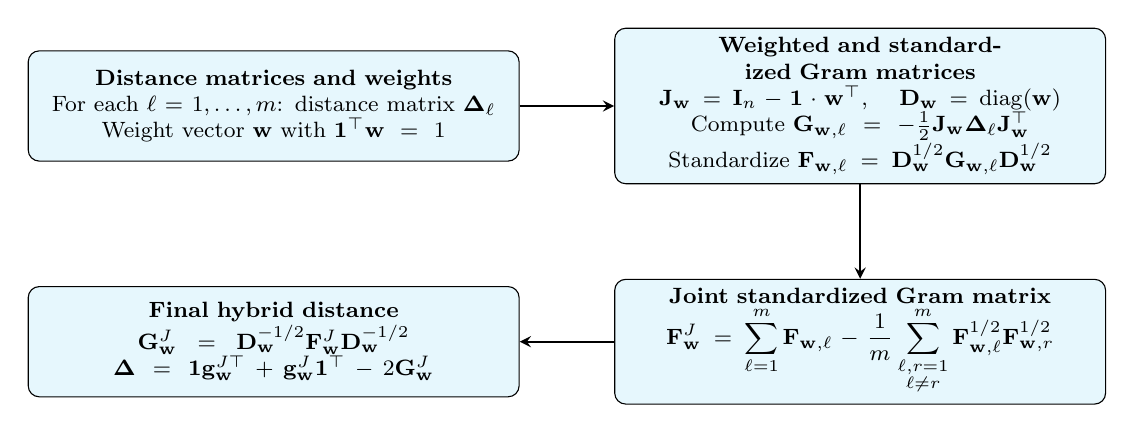
\begin{tikzpicture}[node distance=1.2cm and 1.2cm, >=stealth]
% Node styles
\tikzset{
  box/.style={rectangle, draw, text width=6cm, align=center, rounded corners,
              minimum height=1.4cm, fill=cyan!10, font=\footnotesize},
  arrow/.style={->, thick}
}

% Nodes
\node[box] (A) {
 \textbf{Distance matrices and weights} \\
  For each $\ell = 1,\dots,m$: distance matrix $\mathbf{\Delta}_\ell$ \\
  Weight vector $\mathbf{w}$ with $\mathbf{1}^\top \mathbf{w} = 1$
};

\node[box, right=of A] (B) {
  \textbf{Weighted and standardized Gram matrices} \\
  $\mathbf{J}_\mathbf{w} = \mathbf{I}_n - \mathbf{1}\cdot \mathbf{w}^\top$, \quad $\mathbf{D}_\mathbf{w} = \mathrm{diag}(\mathbf{w})$ \\
  Compute $\mathbf{G}_{\mathbf{w},\ell} = -\frac{1}{2}\mathbf{J}_\mathbf{w} \mathbf{\Delta}_\ell \mathbf{J}_\mathbf{w}^\top$ \\
 Standardize $\mathbf{F}_{\mathbf{w},\ell} = \mathbf{D}_\mathbf{w}^{1/2}\mathbf{G}_{\mathbf{w},\ell}\mathbf{D}_\mathbf{w}^{1/2}$
};

\node[box, below=of B] (C) {
  \textbf{Joint standardized Gram matrix} \\
  $\displaystyle
  \mathbf{F}_\mathbf{w}^J = \sum_{\ell=1}^{m}\mathbf{F}_{\mathbf{w},\ell} - \frac{1}{m}\sum_{\substack{\ell,r=1\\\ell\neq r}}^{m}\mathbf{F}_{\mathbf{w},\ell}^{1/2}\mathbf{F}_{\mathbf{w},r}^{1/2}$
};

\node[box, left=of C] (D) {
  \textbf{Final hybrid distance} \\
  $\mathbf{G}_\mathbf{w}^J = \mathbf{D}_\mathbf{w}^{-1/2}\mathbf{F}_\mathbf{w}^J\mathbf{D}_\mathbf{w}^{-1/2}$ \\
  $\mathbf{\Delta} = \mathbf{1}\mathbf{g}_\mathbf{w}^{J\top} + \mathbf{g}_\mathbf{w}^J\mathbf{1}^\top - 2\mathbf{G}_\mathbf{w}^J$
};

% Arrows
\draw[arrow] (A) -- (B);
\draw[arrow] (B) -- (C);
\draw[arrow] (C) -- (D);
\end{tikzpicture}
\end{figure}

RelMS thus enables the integration of diverse data types into a unified metric framework suitable for visualization and clustering, though a higher computational cost. This is the reason why in \cite{grane2021robust} a simplified version of the above procedure was proposed, called generalized Gower distance (G-Gower), by considering only the first addend of formula~(\ref{eq:combination_standardized_gram_matrices}), which mirrors Gower's formula of simply summing over the distance matrices (here in terms of the standardized Gram matrices).
The construction of a hybrid distance is implemented in function \texttt{robust\_distances()} (see Section 3.3 for details) which enables the methods \texttt{relms} or \texttt{ggower}, for the simplified version.

\subsection*{Adding robustness to the hybrid metric}

As outlined in Section "Distances for mixed-type data",
%~\ref{sec:mixed_type_distances},
Gower's distance is particularly useful for handling mixed-type data (quantitative, binary and multiclass categorical data). However, it also presents some notable limitations, most importantly, its inability to account for correlations among continuous variables and its lack of robustness, which makes it highly sensitive to outliers.

To overcome these limitations, in \cite{boj2024robustification}, a new robust distance was proposed for quantitative variables, which can be incorporated into either G-Gower's distance or the RelMS approach, and is implemented in function \texttt{robust\_distances()}. This new robust approach increases the resistance of the metric to outliers and enhances reliability when integrating mixed-type variables with observation-specific weights.

Specifically, the quantitative component of the hybrid metric is computed as a robust Mahalanobis distance by means of a DB-trimming estimator, introduced in \cite{grane2021robust} for outlier detection in complex datasets, and adapted for weighted data in \cite{boj2024robustification}.
It should be noted that robustness in the current framework is introduced through the continuous component of the mixed-data dissimilarities, using robust Mahalanobis-type distances. Binary and categorical variables are handled through classical similarity and dissimilarity measures.

In particular, let $\Omega = \{1, \ldots n\}$ be the set of units for which the values of $p$ variables are observed, $\mathbf{z}_1, \dots, \mathbf{z}_n \in \mathbb{R}^p$, and form the rows of the data matrix $\mathbf{Z}_{n \times p}$. Consider a distance measure $\delta$ and for all pairs of units in $\Omega$ compute the matrix of squared distances $\mathbf{\Delta} =  \left ( \delta^{2} \left(\mathbf{z}_i, \mathbf{z}_j \right) \right)_{1 \leq i,j \leq n}$. Then, given a new unit $i_0\notin \Omega$, with observed values  $\mathbf{z}_0\in \mathbb{R}^p$, the proximity of $i_0$ to the individuals in $\Omega$ is defined as:
\begin{equation} 
\label{eq:proximity_function}
  \phi(\mathbf{z}_0) = \sum_{i = 1}^{n} w_i \cdot \delta^2 (\mathbf{z}_0, \mathbf{z}_i) - \mathbf{V_\Delta},  
\end{equation}
where $w_i$ denotes the weight associated with unit $i$, and $\mathbf{V_\Delta}$ is the geometric variability of the distance matrix $\mathbf{\Delta}$, as defined in equation~(\ref{eq:geomvar}).

The proximity function (\ref{eq:proximity_function}) is used as a trimming estimator to exclude a fixed proportion $\alpha$ of the most outlying observations according to distance $\delta$. Although equation (\ref{eq:proximity_function}) is defined for a new observation $\mathbf{z}_{0}$, in practice the proximity function is also evaluated for observations belonging to the reference sample. In this case, no leave-one-out procedure is performed; the computation uses the previously obtained distance matrix and the corresponding geometric variability measures. Therefore, when $\mathbf{z}_{0}=\mathbf{z}_i$ for some $i_0 \in \Omega$, the self-distance is equal to zero and is naturally included in the calculation.

With the trimmed sample, the covariance matrix for the quantitative variables is estimated and plugged into the Mahalanobis distance formula. 
The steps to compute the DB robust estimate of the covariance matrix for the quantitative variables are described in Figure~\ref{fig:robust-mahalanobis-workflow}, where $\mathbf{Z}^{p_1}$ denotes the $n \times p_1$ data matrix with the observations for the quantitative variables, and $\alpha$ is the trimming parameter.

\begin{figure}[htbp]
\centering
\caption{Workflow for computing the robust Mahalanobis component for quantitative variables}
\label{fig:robust-mahalanobis-workflow}

\vspace{0.5em}
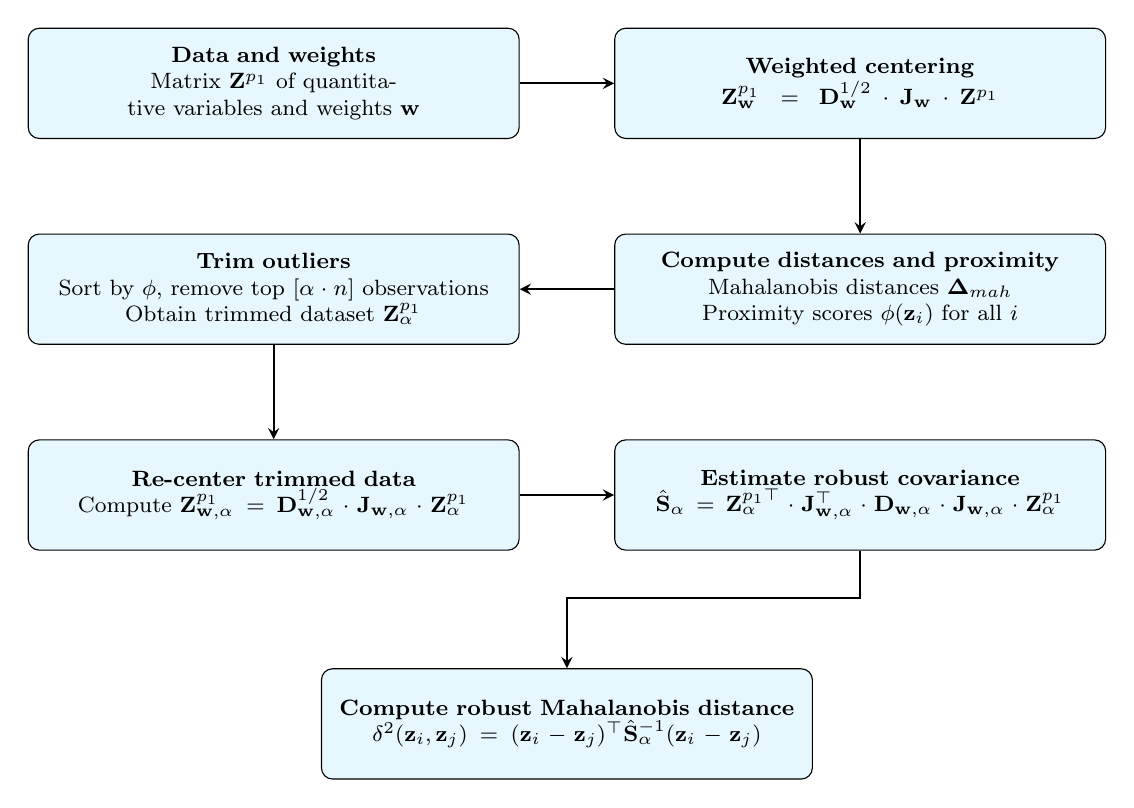
\begin{tikzpicture}[node distance=1.2cm and 1.2cm, >=stealth]
\tikzset{
  box/.style={rectangle, draw, text width=6cm, align=center, rounded corners,
              minimum height=1.4cm, fill=cyan!10, font=\footnotesize},
  arrow/.style={->, thick}
}

% Nodes
\node[box] (A) {
 \textbf{Data and weights} \\
 Matrix $\mathbf{Z}^{p_1}$ of quantitative variables and weights $\mathbf{w}$
};

\node[box, right=of A] (B) {
  \textbf{Weighted centering} \\
  $\mathbf{Z}_{\mathbf{w}}^{p_1} = \mathbf{D}_{\mathbf{w}}^{1/2} \cdot \mathbf{J}_{\mathbf{w}} \cdot \mathbf{Z}^{p_1}$
};

\node[box, below=of B] (C) {
  \textbf{Compute distances and proximity} \\
  Mahalanobis distances $\mathbf{\Delta}_{mah}$ \\
  Proximity scores $\phi(\mathbf{z}_i)$ for all $i$
};

\node[box, left=of C] (D) {
  \textbf{Trim outliers} \\
  Sort by $\phi$, remove top $[\alpha \cdot n]$ observations \\
  Obtain trimmed dataset $\mathbf{Z}_{\alpha}^{p_1}$
};

\node[box, below=of D] (E) {
  \textbf{Re-center trimmed data} \\
  Compute $\mathbf{Z}_{\mathbf{w},\alpha}^{p_1} = \mathbf{D}_{\mathbf{w},\alpha}^{1/2} \cdot \mathbf{J}_{\mathbf{w},\alpha} \cdot \mathbf{Z}_{\alpha}^{p_1}$
};

\node[box, right=of E] (F) {
  \textbf{Estimate robust covariance} \\
 $\hat{\mathbf{S}}_\alpha = \mathbf{Z}_{\alpha}^{p_1\top} \cdot \mathbf{J}_{\mathbf{w},\alpha}^{\top} \cdot \mathbf{D}_{\mathbf{w},\alpha} \cdot \mathbf{J}_{\mathbf{w},\alpha} \cdot \mathbf{Z}_{\alpha}^{p_1}$
};

\path (F) -- (E) coordinate[midway] (midpoint);
\node[box, below=2.2cm of midpoint] (G) {
  \textbf{Compute robust Mahalanobis distance} \\
  $\delta^2(\mathbf{z}_i,\mathbf{z}_j) = (\mathbf{z}_i-\mathbf{z}_j)^\top \hat{\mathbf{S}}_\alpha^{-1} (\mathbf{z}_i-\mathbf{z}_j)$
};

% Arrows
\draw[arrow] (A) -- (B);
\draw[arrow] (B) -- (C);
\draw[arrow] (C) -- (D);
\draw[arrow] (D) -- (E);
\draw[arrow] (E) -- (F);
\draw[arrow] (F.south) -- ++(0,-0.6) -| (G.north);
\end{tikzpicture}
\end{figure}

The latest version of \CRANpkg{dbrobust} includes the wMCD estimator proposed in \cite{Boj2026} as an alternative to the DB-trimming estimator for robust covariance estimation. The wMCD estimator extends the classical Minimum Covariance Determinant (MCD) methodology to the weighted setting and provides a robust covariance estimator that explicitly incorporates sampling weights. Its inclusion is mainly motivated by computational considerations, as it was designed to substantially reduce the computation time required to estimate the covariance matrix, particularly in high-dimensional and large-scale data sets. The robust covariance estimator used within \texttt{robust\_distances()} is specified through the \texttt{cov\_method} argument, where \texttt{"gv"} (the default option) corresponds to the DB-trimming estimator, whereas \texttt{"mcd"} corresponds to the wMCD estimator.

Furthermore, when only continuous variables are present, robust G-Gower reduces to a robust Mahalanobis distance, providing a robust weighted distance measure in its own right. This constitutes a novel contribution of \CRANpkg{dbrobust}, since no other R implementation currently provides robust Mahalanobis distances based on robust covariance estimators that explicitly accommodate sampling weights. Both DB-trimming and wMCD allow the computation of robust weighted Mahalanobis distances, with wMCD offering improved scalability for big data applications.

% %%%%%%%%%%%%%%%%%%%%%%%%%%%%%%%%%%%%%%%%%%%%%%%%%%%%%%%%%%%%%%%%%%%%%%%%%%%%%%%%%%%%%%%%%%%%%
\section{Software implementation: Core functions}
\label{sec.software}

Although R is a powerful and flexible language for statistical computing, it presents notable limitations in DB multivariate analysis. In particular, when working with weighted mixed-type data, we identify several gaps: fragmented distance computation, lack of robust methods and Euclidean corrections, and underdeveloped visualization tools, each hindering effective multivariate analysis. These limitations highlight the need for a unified \CRANpkg{dbrobust} package that consolidates and enhances existing tools.

\subsection{Computing dissimilarities and similarities}

One of the central functions in the \CRANpkg{dbrobust} package is \texttt{calculate\_distances()}, which provides a unified interface for computing pairwise distance or similarity matrices from a data frame or matrix. The function supports a wide range of data types, including binary, categorical, continuous, and mixed-type data, and offers compatibility with multiple well-known distance or similarity measures.

The primary objective of \texttt{calculate\_distances()} is to simplify the computation of distances in datasets of mixed-type by providing a flexible and consistent function. Internally, it delegates computation to specialized functions depending on the selected method, while ensuring a standardized value structure. The internal and logical modular structure of \texttt{calculate\_distances()} can be found in Section 1
%~\ref{AppCalculateDistances}
of the Appendix.
%~\ref{App}.

Supported methods include:
\begin{itemize}
  \item Binary data: Jaccard, Dice, Sokal-Michener, Russell-Rao, Sokal-Sneath, Kulczynski, and Hamming.
  \item Categorical data: Matching coefficient, Cramér-based.
  \item Continuous data: Euclidean, Standardized Euclidean, Manhattan, Minkowski, Canberra, Maximum, Cosine, Correlation, and Mahalanobis.
  \item Mixed-type data: Gower. 
\end{itemize}

Note that Gower is a generalized (aggregated) distance that combines continuous, binary, and categorical variables into a single dissimilarity measure. Although conceptually different from purely numeric or purely binary distances, in \texttt{calculate\_distances()} it is included alongside the other methods to provide a unified interface for the user.

A notable feature is the ability to convert distance matrices into similarity matrices (when applicable), and to optionally square the pairwise distances. The function is also designed with flexibility in its output: users can request either a condensed \texttt{dist} object, a full numeric distance matrix, or a similarity matrix. Moreover, users can select the Minkowski power only if the \texttt{minkowski} method is chosen, via the \texttt{p} argument.

The \texttt{calculate\_distances()} function is a core component of the \CRANpkg{dbrobust} package, providing essential support for subsequent operations. At the same time, its general-purpose nature makes it valuable beyond the scope of the package itself, allowing users to compute versatile distance or similarity matrices that can serve as input for a wide range of external analytical tasks.

The usage of the \texttt{calculate\_distances()} function is:

\begin{verbatim}
calculate_distances(x, method = "gower", output_format = "dist",
                    squared = FALSE, q = NULL, 
                    similarity_transform = "linear", 
                    type = list(),weights = NULL)
\end{verbatim}

where:
\begin{description}
  \item[x:] A matrix or data.frame. Each row represents an observation.
  \item[method:] A string specifying the distance/similarity method. Supported options are:
\begin{itemize}
    \item Binary: \texttt{"jaccard"}, \texttt{"dice"}, \texttt{"sokal\_michener"}, \texttt{"russell\_rao"}, \texttt{"sokal\_sneath"}, \texttt{"kulczynski"}, \texttt{"hamming"}.
    \item Categorical: \texttt{"matching\_coefficient"}, \texttt{"cramer"}.
    \item Continuous: \texttt{"euclidean"}, \texttt{"euclidean\_standardized"}, \texttt{"manhattan"}, \texttt{"minkowski"}, \texttt{"canberra"}, \texttt{"maximum"}, \texttt{"cosine"}, \texttt{"correlation"}, \texttt{"mahalanobis"}.
    \item Mixed: \texttt{"gower"}.
\end{itemize}
	  \item[output\_format:] Output format:  \texttt{"dist"} (distance object), \texttt{"matrix"} (numeric matrix), or \texttt{"similarity"}
    (only for binary/categorical/mixed methods).
    squared Logical; if \texttt{TRUE}, returns squared distances (not applied to similarities).
  \item[squared:] Logical; if \texttt{TRUE}, returns squared distances (not applied to similarities).
  \item[q:] Numeric; the power parameter for the Minkowski distance (required if \texttt{method = "minkowski"}); ignored otherwise.
  \item[similarity\_transform:] Character string; if\texttt{output\_format = "similarity"}, this specifies the formula
to convert distances to similarity scores. Supported: \texttt{"linear"} (default), $s_{ij} = 1-\delta_{ij}$,  or
\texttt{"sqrt"}, $s_{ij} = 1-\delta_{ij}^{2}$.
\item[type] Optional list specifying variable types for Gower distance (passed directly to
\texttt{cluster::daisy}). Arguments can be \texttt{symm}, \texttt{asymm}, \texttt{ordratio}, or \texttt{logratio}.

\item[weights] Optional numeric vector containing weights. Its interpretation depends on the
chosen method:
\begin{description}
      \item[For Gower distance (\texttt{method = "gower"}):] A vector of length \texttt{ncol(x)} to
weight the \textit{variables} (columns).
\item[For Cramér’s V distance (\texttt{method = "cramer"}):] A vector of length \texttt{nrow(x)}
to weight the \textit{observations} (rows), useful for handling class imbalance or
stratified sampling.
    \end{description}

\end{description}

While \texttt{calculate\_distances()} computes distances for various data types, it does not guarantee that the resulting matrices fulfill the Euclidean property. The next section presents \texttt{make\_euclidean()}, a function designed to verify and, if required, correct squared distance matrices to ensure their Euclidean validity.

\subsection{Ensuring Euclideanarity of matrices of pairwise squared distances}

The \texttt{make\_euclidean()} function is designed to verify and, if necessary, transform a matrix of pairwise \emph{squared} distances into a matrix of pairwise squared distances that fulfills the Euclidean property. This correction is important because some analytical methods, such as classical or metric MDS, require the distance values to satisfy this property. Numerical imprecision or certain data transformations may lead to small violations of this condition, which \texttt{make\_euclidean()} can automatically detect and fix.

The function works by computing the weighted Gram matrix
$\mathbf{G}_{\mathbf{w}} = -\frac{1}{2} \mathbf{J}_{\mathbf{w}} \cdot \mathbf{\Delta} \cdot \mathbf{J_\mathbf{w}}^{\top},$ where $\mathbf{\Delta}$ is the matrix of pairwise squared distances, $\mathbf{w}$ is the user-supplied weight vector, and $\mathbf{J_\mathbf{w}} = \mathbf{I_n} - \mathbf{1} \cdot \mathbf{w}^\top$
is the centering matrix defined by the normalized weights. It then checks the eigenvalues of $\mathbf{G}_{\mathbf{w}}$. If the smallest eigenvalue $\lambda_{\min}$ is smaller than a negative tolerance, the function adds a constant shift to all pairwise distances following the method of \cite{lingoes1971some} and \cite{mardia1978some}, ensuring positive semi-definiteness of the Gram matrix.

The usage of the \texttt{make\_euclidean()} function is:

\begin{verbatim}
make_euclidean(D, w = NULL, tol = 1e-10)
\end{verbatim}

where:

\begin{description}
\item[D:] Square matrix of pairwise \emph{squared} distances.
\item[w:] Numeric vector of weights, with length equal to the number of observations. Defaults to a vector of ones.
\item[tol:] Numeric tolerance for detecting negative eigenvalues.
\end{description}

The function returns a list of values containing four main components. The element \texttt{D\_euc} contains the corrected squared distance values, guaranteed to satisfy Euclidean properties after the procedure. The elements \texttt{eigvals\_before} and \texttt{eigvals\_after} provide the eigenvalues of the weighted Gram matrix $\mathbf{G}_{\mathbf{w}}$ before and after correction, respectively, allowing users to assess the magnitude and necessity of the adjustment. Finally, the element \texttt{transformed} is a logical value indicating whether any correction was applied, or if the matrix argument \texttt{D} already fulfilled the Euclidean conditions presented in Section "The Euclidean property".
%~\ref{sec:Euclidean}.
The internal and logical modular structure of function \texttt{make\_euclidean()} can be found in Section 2
%~\ref{AppMakeEuclidean}
of the Appendix.
%~\ref{App}.

Using \texttt{make\_euclidean()} offers several advantages. It ensures that squared distance values are compatible with algorithms relying on Euclidean geometry, thereby preventing failures or distortions in the resulting embeddings. The correction is deliberately minimal (applied only when violation is detected and using the smallest possible shift), thus preserving the original distance structure as much as possible. It is important to note that the function expects squared distances as argument; if only raw distances are available, they should be squared before calling the function. In this context, the \texttt{disttoD2()} function from the \CRANpkg{dbstats} package can be used to conveniently convert a \texttt{dist} object into a matrix of pairwise squared distances $\mathbf{\Delta}$ before applying \texttt{make\_euclidean()}.

\subsection{Computing robust distances}

The \texttt{robust\_distances()} function is a core component of the \CRANpkg{dbrobust} package, designed to compute robust squared (or simple) distance values between individuals in a weighted dataset containing quantitative, binary, and multiclass categorical variables. It supports two robust distance measures, G-Gower and RelMs described in Section 2.3,
%~\ref{sec:RelMS_space_construction}
and incorporates a DB-trimming procedure for estimating robust covariance matrices in the continuous subspace as was detailed in Figure~\ref{fig:robust-mahalanobis-workflow}.

The usage of the \texttt{robust\_distances()} function is:

\begin{verbatim}
robust_distances(data = NULL, cont_vars = NULL, bin_vars = NULL, 
                 cat_vars = NULL, w = NULL, p = NULL, 
                 method = c("ggower", "relms"), 
                 cov_method = c("gv", "mcd"), 
                 robust_cov = NULL, 
                 alpha = 0.1, niter = 40,
                 nstart = 20, return_dist = FALSE)
\end{verbatim}
where:
\begin{description}
\item[data:] Matrix or data frame containing the data.
\item[cont\_vars, bin\_vars, cat\_vars:] Character vectors of variable names for continuous, binary and categorical respectively (if p is not provided).
\item[w:] Numeric vector of observation weights. If \texttt{NULL}, uniform weights are used.
\item[p:] Integer vector of length 3 with the number of continuous, binary, and multiclass categorical variables (only if columns are sorted in this order).
\item[method:] Aggregation method: \texttt{"ggower"} for robust G-Gower distance values and 
    \texttt{"relms"} for robust RelMS distance values. Defaults to \texttt{"ggower"}.
\item[cov\_method:] Character string specifying the robust covariance method for continuous variables:
either \texttt{"gv"} (Geometric Variability) for the DB-trimming or \texttt{"mcd"} (Minimum Covariance Determinant) for the wMCD trimming algorithm.
Default is "gv".
\item[robust\_cov:] Optional precomputed robust covariance matrix for quantitative variables.
\item[alpha:] Trimming proportion for robust covariance estimation in quantitative variables. Defaults to \texttt{0.1}.
\item[niter:] Integer specifying the number of concentration steps (C-steps) per start. Only
used if \texttt{cov\_method = "mcd"}. Defaults to \texttt{40}.
\item[nstart:] Integer specifying the number of random initializations. Only used if \texttt{cov\_method
= "mcd"}. Defaults to \texttt{20}.
\item[return\_dist:] Logical. If \texttt{TRUE}, returns the distance matrices $\mathbf{D}$ as \texttt{dist} objects; if \texttt{FALSE}, returns squared distance matrices $\mathbf{\Delta}$ as \texttt{D2} objects. Defaults to \texttt{FALSE}.
\end{description}

The internal and logical modular structure of function \texttt{robust\_distances()} can be found in Section 3
%~\ref{AppRobustDistances}
of the Appendix.
%~\ref{App}.

This function is the most critical component of \CRANpkg{dbrobust}, as it operationalizes the novel concepts introduced in \cite{boj2024robustification} and \cite{Boj2026}, which underpin the methodological framework of our current research line. By implementing these ideas within a robust and flexible mixed-data framework, \texttt{robust\_distances()} bridges recent theoretical advances with practical computational tools, enabling their direct application.

{\subsection{Aggregating dissimilarities}}
The \texttt{merge\_distances()} function is a core component of the \CRANpkg{dbrobust} package, designed to combine multiple distance matrices into a single consensus distance matrix that fulfills the Euclidean property. The aggregation can be performed either through a direct weighted combination of distances based on a Pythagorean sum (Gower-like approach) or through RelMS, which accounts for redundancy among sources (see Figure~\ref{fig:relms-workflow-general-weighted}). The procedure accommodates both source-specific weights, controlling the contribution of each distance matrix to the consensus solution, and sampling weights associated with the observations. In all cases, input and output distance matrices are enforced to fulfill the Euclidean requirement through \texttt{make\_euclidean()}.

The usage of the \texttt{merge\_distances()} function is: 

\begin{verbatim} 
merge_distances(distance_list, matrix_weights = NULL,  w = NULL,
                squared = FALSE, RelMS = TRUE, tol = 1e-10 ) 
\end{verbatim} 
where: 
\begin{description}
\item[distance\_list:] A list of distance matrices or \texttt{dist} objects. All distance matrices must be square (\(n \times n\)) and correspond to distances that fulfill the Euclidean property. 
\item[matrix\_weights:] Numeric vector of weights associated with the distance matrices in \texttt{distance\_list}. Weights must be strictly positive and sum to one. If \texttt{NULL}, all matrices receive equal weight. 
\item[w:] Optional numeric vector of observation weights. Weights must be strictly positive and are normalized to sum to one. If \texttt{NULL}, uniform weights are assumed. 
\item[squared:] Logical value indicating whether the input matrices contain squared distances. If \texttt{FALSE} (default), distances are squared internally during the aggregation process. If \texttt{TRUE}, inputs are treated as already squared. 
\item[RelMS:] Logical value indicating the aggregation method. If \texttt{TRUE} (default), aggregation is performed using RelMS, which penalizes redundancy among distance matrices. If \texttt{FALSE}, a direct weighted combination based on a Pythagorean sum is computed. 
\item[tol:] Numeric tolerance used by \texttt{make\_euclidean()} when enforcing the Euclidean property through eigenvalue decomposition. Defaults to \texttt{1e-10}. 
\end{description}

In the latest version of \CRANpkg{dbrobust}, the \texttt{merge\_distances()} function has been added as a general framework for distance aggregation. Besides enabling the application of RelMS to the classical Gower approach for mixed data, it allows the combination of any set of distance matrices, whether derived from different variable blocks, different distance measures, or externally provided dissimilarity data, providing a flexible and widely applicable distance integration strategy.

The details of the modular structure can be found in Section 4 
%~\ref{AppVisualizeDistances}
of the Appendix.

\subsection{Visualizing distances and similarities}

Visualizing relationships in distance matrices remains limited in R. Tools such as \texttt{qgraph()} from the \CRANpkg{qgraph} package \citep{qgraph} and \texttt{ggpairs()} from the \CRANpkg{GGally} package \citep{GGally} offer partial solutions, but lack integration with MDS configurations, scale poorly with mixed-type data, and provide limited customization for grouped or weighted analyses. In particular, conditional visualizations, faceted MDS plots, and DB heatmaps or network representations are not natively supported in a cohesive and user-friendly manner.

The functions \texttt{cmdscale()} and \texttt{wcmdscale()}, which perform classical and weighted MDS respectively, do not internally verify whether the distance matrix passed as an argument fulfills the Euclidean requirement. In particular, they do not check the positive semi-definiteness of the associated Gram matrix constructed via double centering of the squared distances. If the Gram matrix is not positive semi-definite, the distance matrix does not fulfill the Euclidean property, and the MDS embedding may produce invalid or complex (imaginary) coordinates.

The \texttt{visualize\_distances()} function in the \CRANpkg{dbrobust} package provides a versatile interface to explore and display distances or similarities through various visualization techniques. It supports multiple plotting methods including classical and weighted MDS, heatmaps, and network graphs.

This function accepts distance matrices in either \texttt{dist} objects or symmetric square matrices \texttt{D2}, performing argument validation to ensure correctness. It offers flexibility in the number of dimensions for MDS (parameter \texttt{k}), optional weighting schemes, and grouping variables to color or annotate observations. Supported visualization methods include:
\begin{itemize}
    \item Classic MDS: Classic MDS from \texttt{R} base function \texttt{cmdscale},
    \item Weighted MDS: Weighted MDS variant implemented using the \texttt{wcmdscale()} function from the \CRANpkg{vegan} package,
    \item Heatmap: Displays pairwise distances as a colored matrix with optional grouping and clustering, and
    \item Network graph: Visualizes relationships as a network using the \CRANpkg{qgraph} package.
\end{itemize}

The usage of the \texttt{visualize\_distances()} function is:

\begin{verbatim}
visualize_distances(dist_mat, method = c("mds_classic", "mds_weighted", 
                    "heatmap", "qgraph"), k = 3, weights = NULL, 
                    group = NULL, group_colors = NULL,
                    main_title = NULL, tol = 1e-10, ...)

\end{verbatim}
where:
\begin{description}
\item[dist\_mat:] Square distance matrix (numeric) or a \texttt{dist} object containing pairwise
distances between individuals.
\item[method:] Character string specifying the visualization method: \texttt{"mds\_classic"}, \texttt{"mds\_weighted"}, \texttt{"heatmap"}, or \texttt{"qgraph"}. Defaults to \texttt{"mds\_classic"}.
\item[k:] Integer. Number of dimensions for MDS (default \texttt{3}). Must satisfy $1 \le k \le \min(4, n_{\text{obs}}-1)$.
\item[weights:] Optional numeric vector of weights for weighted MDS. The dimension must match the number
of observations. Defaults to a vector of ones.
\item[group:] Optional factor or vector indicating group membership for coloring or annotating
observations.
\item[group\_colors:] Optional character vector of custom colors for the groups. If \texttt{NULL}, a predefined custom palette is used.
\item[main\_title:] Optional character string specifying the main plot title.
\item[tol:] Numeric tolerance for checking approximate symmetry and Euclidean property. Defaults to  \texttt{1e-10}.
\item[\ldots] Additional arguments passed to internal plotting functions (\texttt{plot\_mds}, \texttt{plot\_heatmap}, or \texttt{plot\_qgraph}), such as clustering method, palette, max nodes, edge thresholds, etc.
\end{description}

The modular design makes \texttt{visualize\_distances()} maintainable, extensible, and easy to understand. By delegating specific tasks to helper functions, each visualization method is implemented independently, which simplifies future extensions and maintenance. The details of the modular structure can be found in Section 5
%~\ref{AppVisualizeDistances}
of the Appendix.
%~\ref{App}.

The function \texttt{visualize\_distances} does not automatically enforce Euclidean geometry. However, users who need a Euclidean embedding can preprocess their distance matrix using the function \texttt{make\_euclidean}, which inspects the Gram matrix and optionally applies an eigenvalue correction (as detailed in Section 2.3).
%~\ref{sec:RelMS_space_construction})
This ensures that the resulting MDS embedding is valid and interpretable in a Euclidean space.

% %%%%%%%%%%%%%%%%%%%%%%%%%%%%%%%%%%%%%%%%%%%%%%%%%%%%%%%%%%%%%%%%%%%%%%%%%%%%%%%%%%%%%%%%%%%%%

\subsection{Interoperability with the R ecosystem}
Beyond its compatibility with the \CRANpkg{dbstats} package, the dissimilarities computed by \CRANpkg{dbrobust}, which can be represented as \texttt{dist} objects, can be directly employed by a broad range of DB procedures available in R. These include hierarchical and partitioning clustering methods such as \texttt{hclust()} from \CRANpkg{stats} and \texttt{agnes()}, \texttt{diana()}, \texttt{pam()}, \texttt{fanny()}, and \texttt{clara()} from \CRANpkg{cluster}. They can also be used in ordination techniques, including classical multidimensional scaling via \texttt{cmdscale()} from \CRANpkg{stats}, non-metric multidimensional scaling via \texttt{isoMDS()} from \CRANpkg{MASS} and \texttt{metaMDS()} from \CRANpkg{vegan}, and principal coordinates analysis via \texttt{pcoa()} from \CRANpkg{ape} \citep{ape}. Furthermore, the resulting dissimilarities can serve as input for inferential procedures such as PERMANOVA through \texttt{adonis2()}, ANOSIM through \texttt{anosim()}, Mantel tests through \texttt{mantel()}, and DB redundancy analysis through \texttt{capscale()}, all available in \CRANpkg{vegan}. Additional examples are summarized in Table~\ref{tab:interoperability}, which highlights the breadth of DB methods that can directly operate on dissimilarities generated by \CRANpkg{dbrobust}. Consequently, \CRANpkg{dbrobust} may be viewed not only as a tool for robust distance computation but also as a general-purpose provider of dissimilarity measures that can be readily integrated into a wide variety of statistical learning, exploratory data analysis, and DB modelling workflows within the R ecosystem.

\begin{table}[h!] 
\centering 
\caption{Examples of downstream methods accepting \texttt{dist} objects generated from \CRANpkg{dbrobust}.} 
\label{tab:interoperability}
\begin{tabular}{@{}p{3.5cm}p{3.5cm}p{5.5cm}@{}} 
\hline 
Method category & Package & Functions \\
 \hline 
Hierarchical clustering & \CRANpkg{stats}, \CRANpkg{cluster} & \texttt{hclust()}, \texttt{agnes()}, \texttt{diana()} \\ 
Partitioning clustering & \CRANpkg{cluster} & \texttt{pam()}, \texttt{fanny()}, \texttt{clara()} \\ 
Ordination & \CRANpkg{stats}, \CRANpkg{MASS}, \CRANpkg{vegan}, \CRANpkg{ape} & \texttt{cmdscale()}, \texttt{isoMDS()}, \texttt{metaMDS()}, \texttt{pcoa()} 
\\ DB inference & \CRANpkg{vegan} & \texttt{adonis2()}, \texttt{anosim()}, \texttt{mantel()}, \texttt{capscale()} 
\\ DB modelling & \CRANpkg{dbstats} & \texttt{dblm()}, \texttt{dbglm()}, \texttt{dbplsr()}, \texttt{ldblm()}, \texttt{ldbglm()} \\ 
\hline 
\end{tabular} 
\end{table}

\section{Examples}
\label{sec.examples}

%In this section, we analyze two mixed-type datasets to illustrate some of the functionalities of the \texttt{dbrobust} package. 
In this section, we analyze two mixed-type datasets to illustrate different functionalities of the \CRANpkg{dbrobust} package. The simulated dataset is used to highlight the behavior of the proposed methodologies under controlled contamination settings, whereas the real-data application serves as a practical vignette illustrating the package workflow and its main functions.
In both cases, we start by computing three different metrics: classical Gower, robust G-Gower and robust RelMS, by means of functions \texttt{calculate\_distances()} using \texttt{method = "gower"} (the default option) and \texttt{robust\_distances()} with \texttt{method = "ggower"} or \texttt{method = "relms"}. For the robust metrics, the sample covariance matrix required in the Mahalanobis distance is estimated using DB-trimming (\texttt{cov\_method = "gv"}, the default option) with a trimming parameter of \texttt{alpha = 0.1} (the default value).
The next step is to assess the Euclideanarity condition, and for that purpose function \texttt{make\_euclidean()} is applied to the three distance matrices. Finally, we proceed by comparing their Euclidean configurations with multiple MDS plots, as well as a direct comparison by means of network representations. For that purpose, the \texttt{visualize\_distances()} function is used as a powerful tool for uncovering patterns and anomalous data through the visual inspection of dissimilarities between units.

\subsection{Simulated data}
The package \texttt{dbrobust} contains four sets of simulated data called \texttt{Data\_HC\_no\_contamination}, \texttt{Data\_HC\_contamination}, \texttt{Data\_MC\_no\_contamination} and \texttt{Data\_MC\_contamination}. All of them were generated from multivariate normal distributions with $p = 9$ components, and different patterns of underlying correlation (high/moderate). The first four components were retained in the continuous form, while the remaining dimensions were later discretized into binary or multiclass categorical variables using percentile-based thresholds. Finally, a 5\%-outlying contamination was added to some of the continuous components (see \citealp{boj2024robustification} for the details).

In addition to the original variables, each dataset incorporates a weighting variable containing the weights for each observation, specifically constructed to illustrate the methodology with weights. To create the weighting variable, a proportional frequency-based approach derived from the joint distribution of the first multiclass and the first binary variables was adopted.

In this section, we focus on the dataset \texttt{Data\_MC\_contamination} to illustrate some of the functionalities of the \texttt{dbrobust} package. In particular, this dataset is composed of 525 observations and 9 variables of mixed type (4 continuous, 3 multiclass categorical, and 2 binary), with an underlying moderate correlation structure ($\rho = 0.6$) as well as the weights. The last 25 rows correspond to contaminated observations created by adding perturbations equal to three times the standard deviation of each quantitative variable to a subset of the 500 original units.

We present a comparative study of three distance metrics: the classical Gower and two robust alternatives, G-Gower and RelMS. The goal of this comparison is to evaluate the effectiveness of robust methods under realistic conditions involving data contamination.

The analysis begins with a qualitative exploration using classical MDS configurations to visualize how each metric captures the underlying data structure (see Figure~\ref{fig:all_visuals2}, where option \texttt{"mds\_classic"} was used to produce the conditional multiple MDS plot and outlying units were identified with the \texttt{"group"} option). The classical Gower metric (panel~\ref{fig:gower_mc}) exhibits a pronounced artifact caused by binary and categorical variables, which severely degrades the visualization. This discretization leads to an artificial stratification of the data into three distinct bands, obscuring the underlying continuous relationships among observations. In contrast, both robust metrics, G-Gower (panel~\ref{fig:ggower_mc_to}) and RelMS (panel~\ref{fig:relms_mc_to}), successfully separate the outlying observations from the main data cloud, placing them clearly apart from the bulk of the data. This effect results from the robust Mahalanobis distance used for continuous predictors in G-Gower and the combined treatment of variable types in RelMS, which integrates robust Mahalanobis, Jaccard and Hamming distances for continuous, binary, and multiclass predictors, respectively.

Panels~\ref{fig:ggower_mc_to}--\ref{fig:relms_mc_to} show the true outliers (known from the data generation process) for comparison. The visual agreement between outliers detected in the trimming step (panels~\ref{fig:ggower_mc}--\ref{fig:relms_mc}) and true outliers confirms the good sensitivity of the robust methods. Overall, the robust configurations reveal not only a better isolation of anomalous units but also a clearer depiction of the underlying clustered structure among regular observations, an effect that is masked under the classical Gower metric.

\begin{figure}[!htbp]
\centering
\begin{subfigure}[b]{0.32\linewidth}
    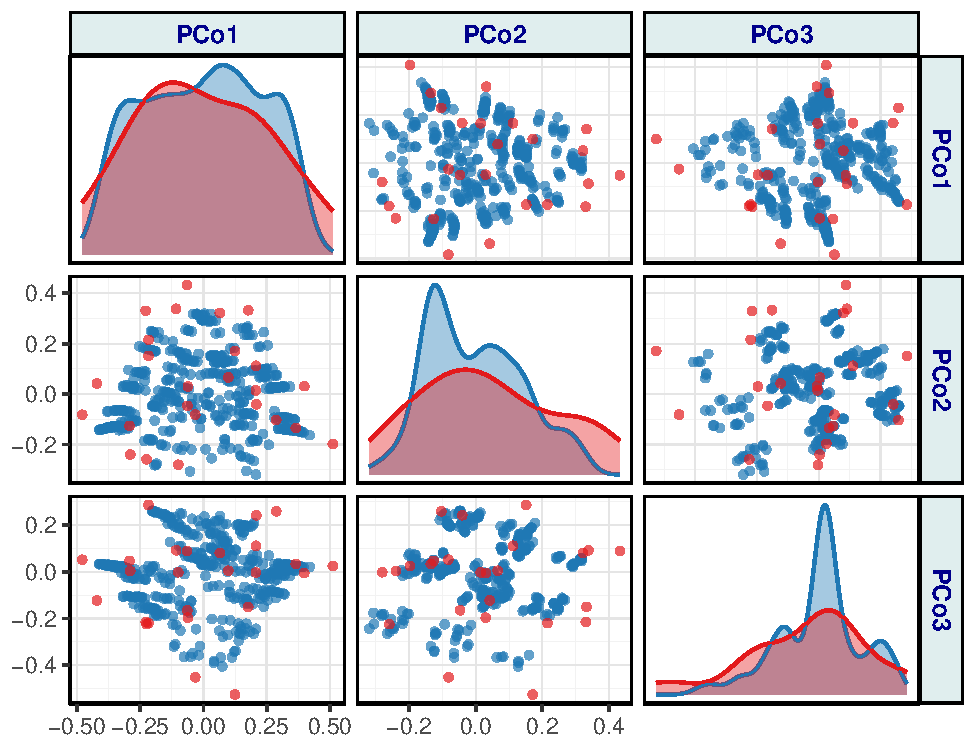
\includegraphics[width=\linewidth]{imagenes/MDSMCCGower.pdf}
    \caption{\footnotesize{Gower (outlying units)}}
    \label{fig:gower_mc}
\end{subfigure}
\begin{subfigure}[b]{0.32\linewidth}
    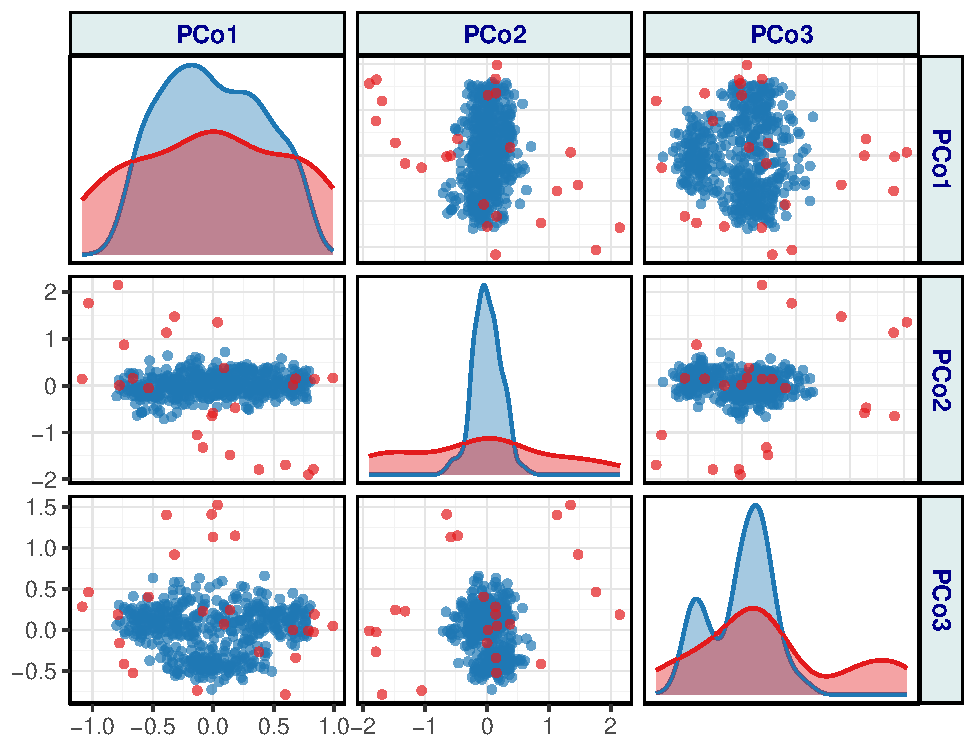
\includegraphics[width=\linewidth]{imagenes/MDSMCCGGowerOut.pdf}
    \caption{\footnotesize{G-Gower (outlying units)}}
    \label{fig:ggower_mc_to}
\end{subfigure}
\begin{subfigure}[b]{0.32\linewidth}
    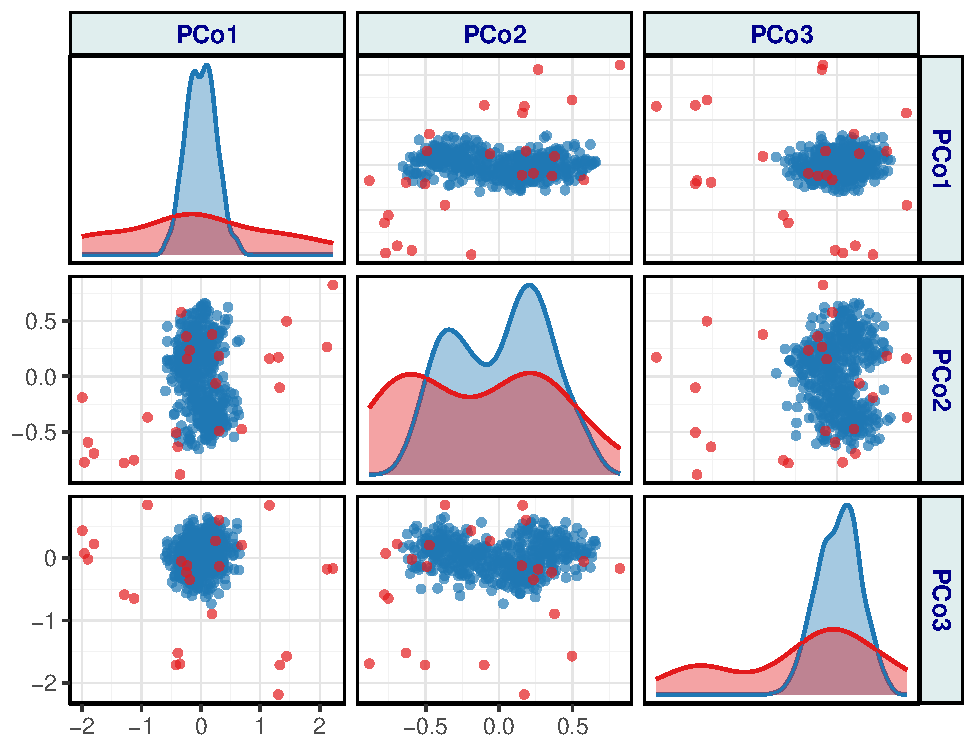
\includegraphics[width=\linewidth]{imagenes/MDSMCCRelMSOut.pdf}
    \caption{\footnotesize{RelMS (outlying units)}}
    \label{fig:relms_mc_to}
\end{subfigure}

\vspace{0.3cm}

\begin{subfigure}[b]{0.32\linewidth}
    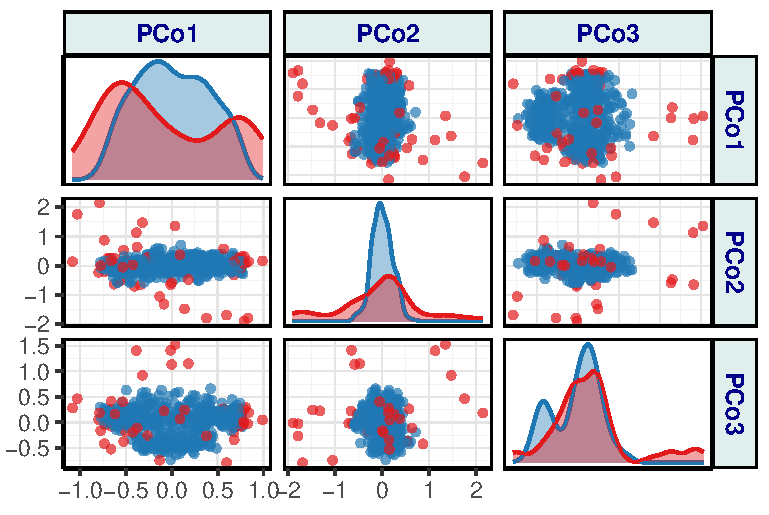
\includegraphics[width=\linewidth]{imagenes/MDSMCCGGower.pdf}
    \caption{\footnotesize{G-Gower (trimmed units)}}
    \label{fig:ggower_mc}
\end{subfigure}
\begin{subfigure}[b]{0.32\linewidth}
    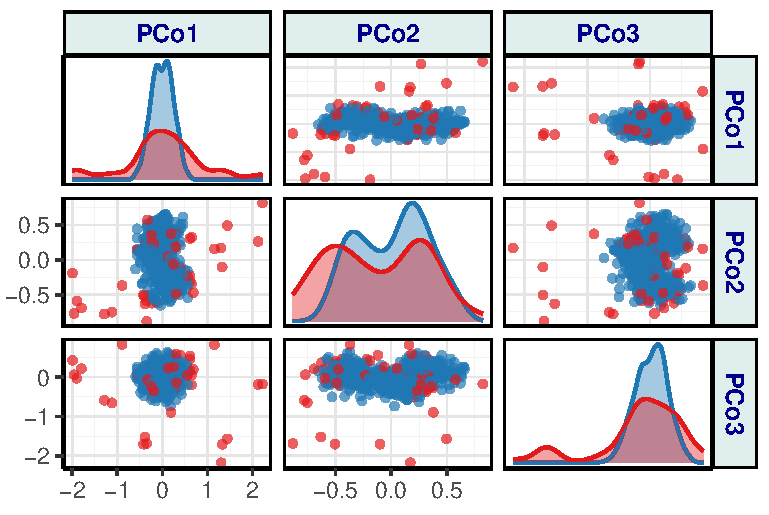
\includegraphics[width=\linewidth]{imagenes/MDSMCCRelMS.pdf}
    \caption{\footnotesize{RelMS (trimmed units)}}
    \label{fig:relms_mc}
\end{subfigure}

\caption{MDS configurations for the \texttt{Data\_MC\_contamination} dataset. Panels (a)--(c) display the configurations obtained using the Gower, G-Gower, and RelMS distances, respectively, where red points correspond to the true outliers introduced in the data generation process. In panels (d)--(e) highlighted points indicate the trimmed units to estimate the covariance matrix in Mahalanobis distance.}
\label{fig:all_visuals2}
\end{figure}

The analysis is followed by an examination of similarity networks to provide a more detailed view of the relationships among observations. Figure~\ref{fig:qgraphs_mc} displays the similarity networks (produced with \texttt{"qgraph"} option of function \texttt{visualize\_distances()}), where each node represents an observation, and spatial proximity between nodes reflects pairwise similarity (obtained as $1-\delta$, where $\delta$ is the distance measure): nodes positioned closer together correspond to more similar observations, while those farther apart are more dissimilar. For visualization purposes, the graphs show randomly selected stratified subsamples of $100$ observations, preserving the target outlier proportions. Outlying units are colored red.

\begin{figure}[!htbp]
\centering
    % --- Fila única: 3 imágenes ---
    \begin{subfigure}{0.32\textwidth}
        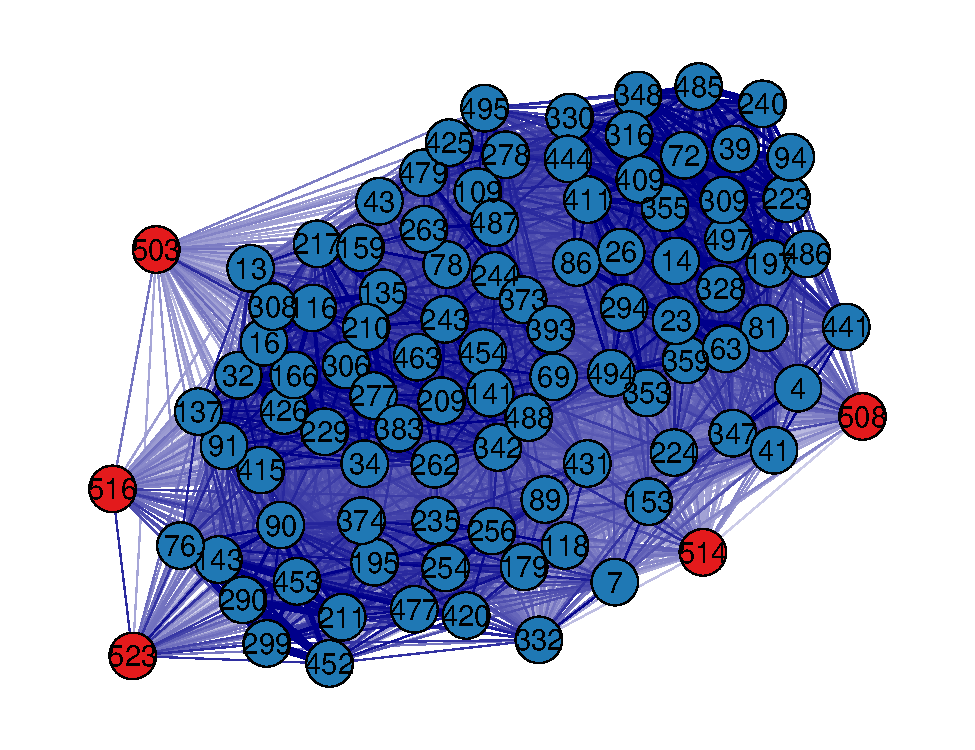
\includegraphics[width=\linewidth]{imagenes/QgraphMCCGower.pdf}
        \caption{\footnotesize{Gower (outlying units)}}
        \label{fig:qgraph_gower_mc}
    \end{subfigure}
    \begin{subfigure}{0.32\textwidth}
        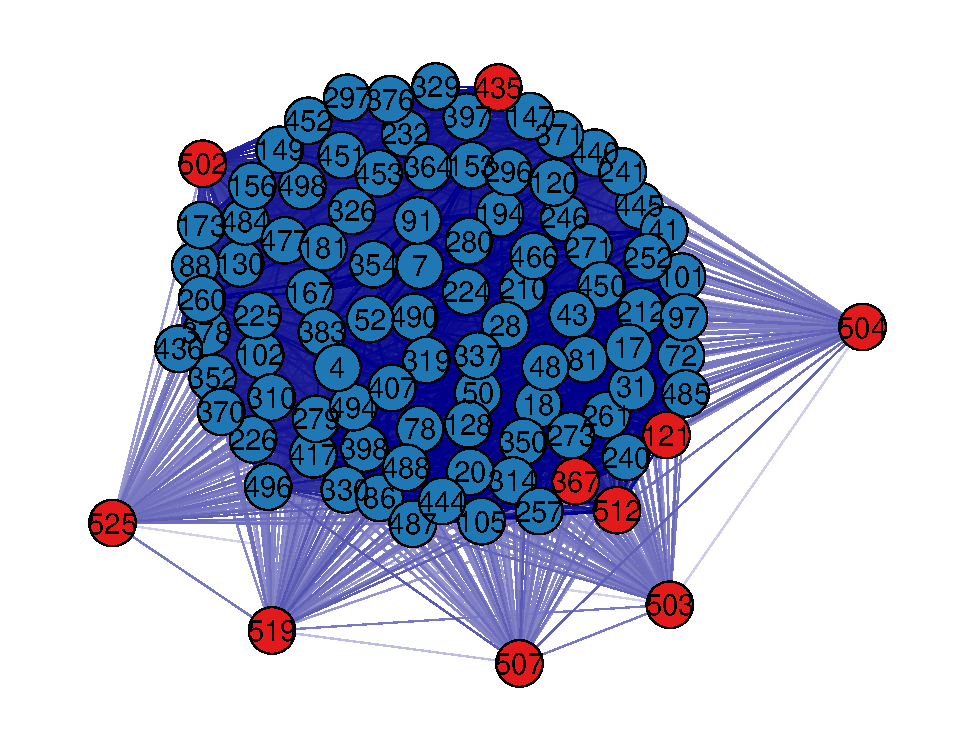
\includegraphics[width=\linewidth]{imagenes/QgraphMCCGGower.pdf}
        \caption{\footnotesize{G-Gower (trimmed units)}}
        \label{fig:qgraph_ggower_mc}
    \end{subfigure}
    \begin{subfigure}{0.32\textwidth}
        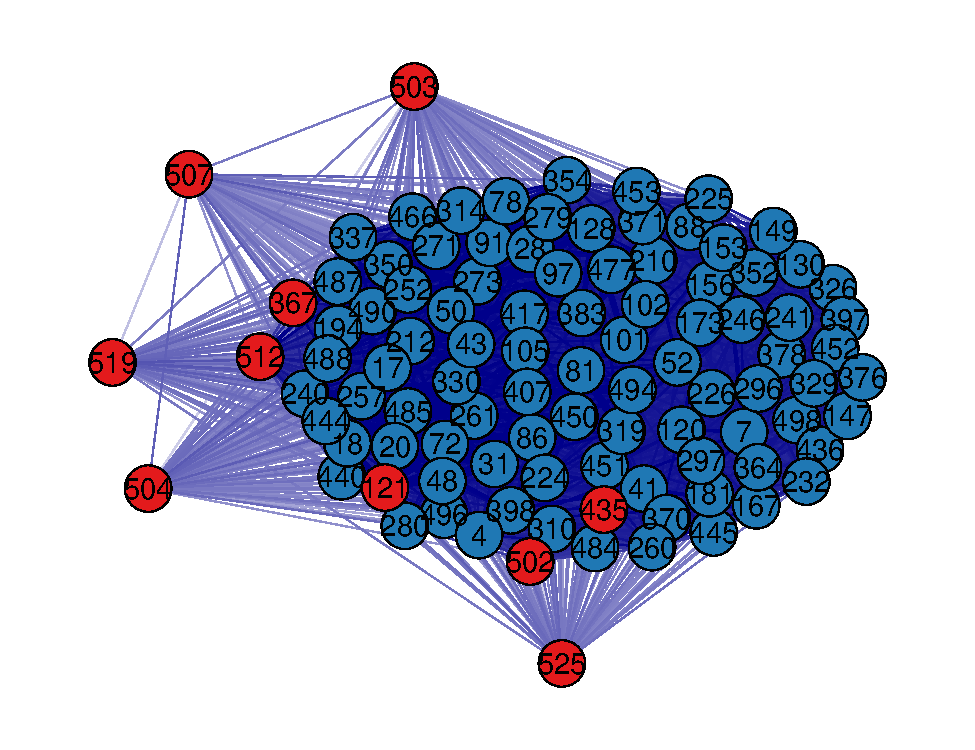
\includegraphics[width=\linewidth]{imagenes/QgraphMCCRelMS.pdf}
        \caption{\footnotesize{RelMS (trimmed units)}}
        \label{fig:qgraph_relms_mc}
    \end{subfigure}

    \vspace{0.3cm}

    % --- Fila inferior: 2 imágenes ---
    \begin{subfigure}{0.32\textwidth}
        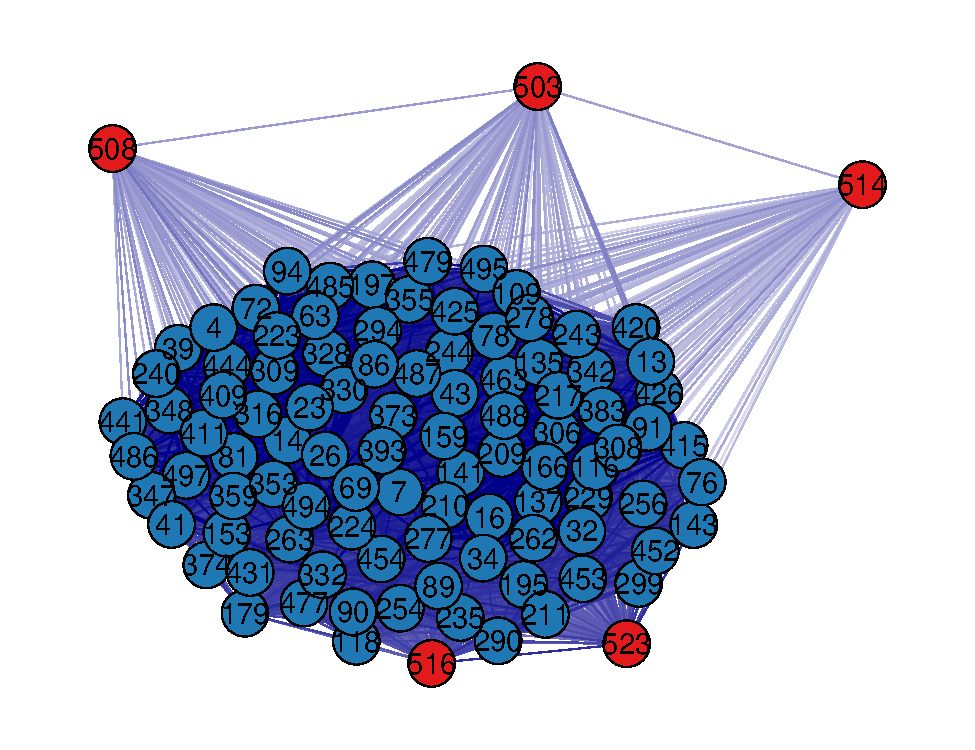
\includegraphics[width=\linewidth]{imagenes/QgraphMCCGGowerOut.pdf}
        \caption{\footnotesize{G-Gower (outlying units)}}
        \label{fig:qgraph_ggower_mc_to}
    \end{subfigure}
    \begin{subfigure}{0.32\textwidth}
        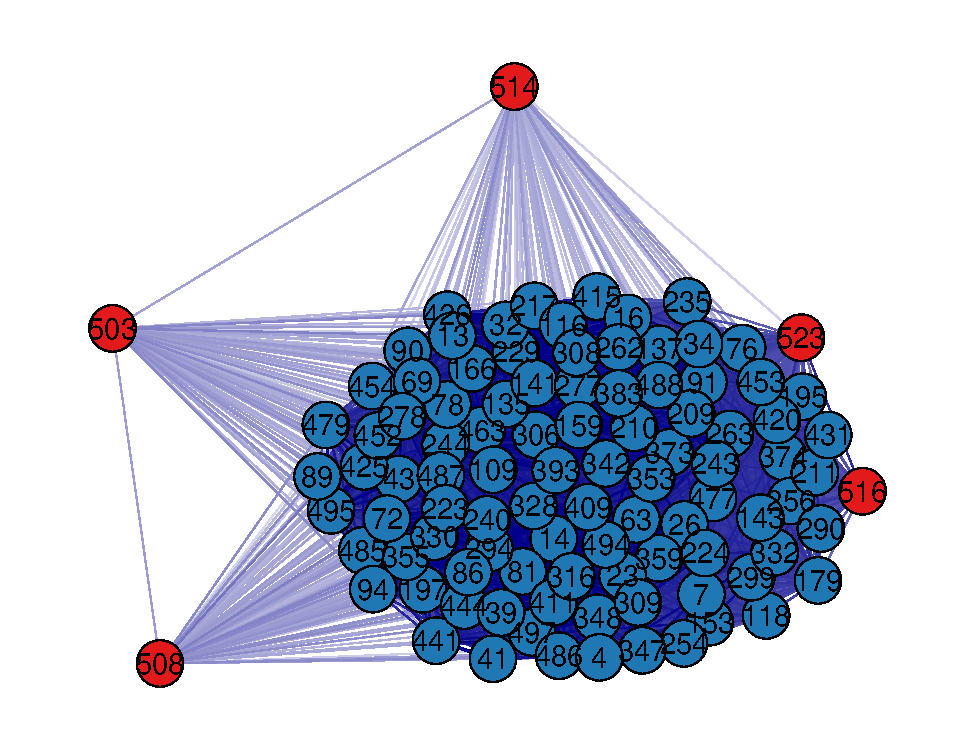
\includegraphics[width=\linewidth]{imagenes/QgraphMCCRelMSOut.pdf}
        \caption{\footnotesize{RelMS (outlying units)}}
        \label{fig:qgraph_relms_mc_to}
    \end{subfigure}

\caption{Similarity networks (qgraphs) for the \texttt{Data\_MC\_contamination} dataset. 
Panels (a)--(c) display the connectivity structure of the observations under the Gower, G-Gower, and RelMS distance measures, respectively. In panel (a), red nodes correspond to the true outliers introduced during data generation, 
whereas in panels (b) and (c), red nodes indicate the outliers detected by the trimming procedure. Panels (d)--(e) show the true outliers for G-Gower and RelMS, respectively, to facilitate comparison between detected and actual anomalous units.}
\label{fig:qgraphs_mc}
\end{figure}

A clear visual pattern emerges: many red nodes are either clustered together or separated from the main cloud of blue nodes (non-outliers). Even when red nodes are not distinctly isolated, they tend to appear on the periphery of the blue cloud and are often connected to other red nodes. Furthermore, since the true outliers were placed as the last observations (indices $>500$), visual inspection reveals that many of the trimmed nodes correspond to this upper-index region, confirming that the trimming procedure effectively captures a substantial proportion of the true outliers.

It is worth emphasizing, however, that the trimming step implemented in the robust distances is not primarily intended as an outlier detection procedure. Its goal is to robustify the distance estimation by reducing the influence of observations that lie far from the bulk of the data, rather than to explicitly identify or label them as anomalous. The fact that many trimmed units coincide with the true outliers illustrates the effectiveness of this robustification process: by downweighting or excluding extreme observations, the robust distances recover a more faithful representation of the underlying data geometry.

Overall, the visual evidence provided by the MDS configurations and similarity networks generated using the \texttt{visualize\_distances()} function from the \texttt{dbrobust} package suggests that the robust metrics are effective in isolating anomalous observations while preserving the structure of the regular data, thereby achieving a more reliable foundation for subsequent modeling or clustering tasks.

\subsection{World development indicators}

To illustrate the performance of the robust distance measures in a real-world setting, we analyze a dataset derived from the \textit{World Development Indicators} (World Bank), available at {\small \url{https://www.kaggle.com/datasets/hn4ever/world-development-indicators-bycountries}}. The dataset comprises a set of socioeconomic indicators that capture diverse dimensions of national development with a sample size of 97 countries worldwide. Specifically, we use the observations corresponding to the year 2021, which is the latest year consistently available for the selected indicators. The numerical variables include the homicide rate (\texttt{Hom}, number of homicides per 100,000 inhabitants), the proportion of the population living on less than \$3.20 per day adjusted for purchasing power parity (\texttt{B320}), life expectancy at birth (\texttt{LEx}), infant mortality rate (\texttt{IMo}, number of children dying before age one per 1,000 live births), the percentage of the population suffering from insufficient nutrition (\texttt{INu}), government expenditure on education as a percentage of GDP (\texttt{GEE}), and the proportion of arable land suitable for cultivation (\texttt{ArL}).
Three binary variables describe key aspects of infrastructure and public services: the adequacy of the health system (\texttt{HSy}, with categories 1 = Adequate, 2 = Inadequate), access to electricity (\texttt{Ele}, with categories 1 = High, 2 = Low) and the poverty indicator (\texttt{Pov}, with two categories: 1 = High and 2 = Low) that classifies countries according to their general poverty status.
In addition, two categorical variables provide contextual information: the continent of each country (\texttt{Con}, with five categories: Africa, Americas, Asia, Europe, and Oceania) and the pollution level (\texttt{Pol}, with three categories: 1 = High, 2 = Medium, 3 = Low).

It is important to note that the variables \texttt{Con} (Continent) and \texttt{Pov} (Poverty) were not included in the distance computation, as they were used exclusively for conditioning and interpretative purposes in the subsequent analyses.

Additionally, to account for the relative importance of each observation, a weighting variable was incorporated into the dataset based on national population size. Specifically, total population data for the most recent available year (2022) were retrieved from the DataHub repository (sourced from the World Bank). The resulting population figures were merged with the main dataset by country name, and normalized to create observation-specific weights. These weights reflect the demographic scale of each country and are employed in subsequent analyses to ensure that larger populations exert proportionally greater influence while preserving comparability among units.

To analyze this mixed-type dataset, we proceed as in the previous application. We start by computing the three distances, namely Gower, robust G-Gower and robust RelMS, and before their comparison, we include a heatmap representation for robust G-Gower metric (produced with \texttt{"heatmap"} option) for illustrative purposes (see Figure~\ref{fig:heatmap.ggower}).

\begin{figure}[h!]
    \centering
    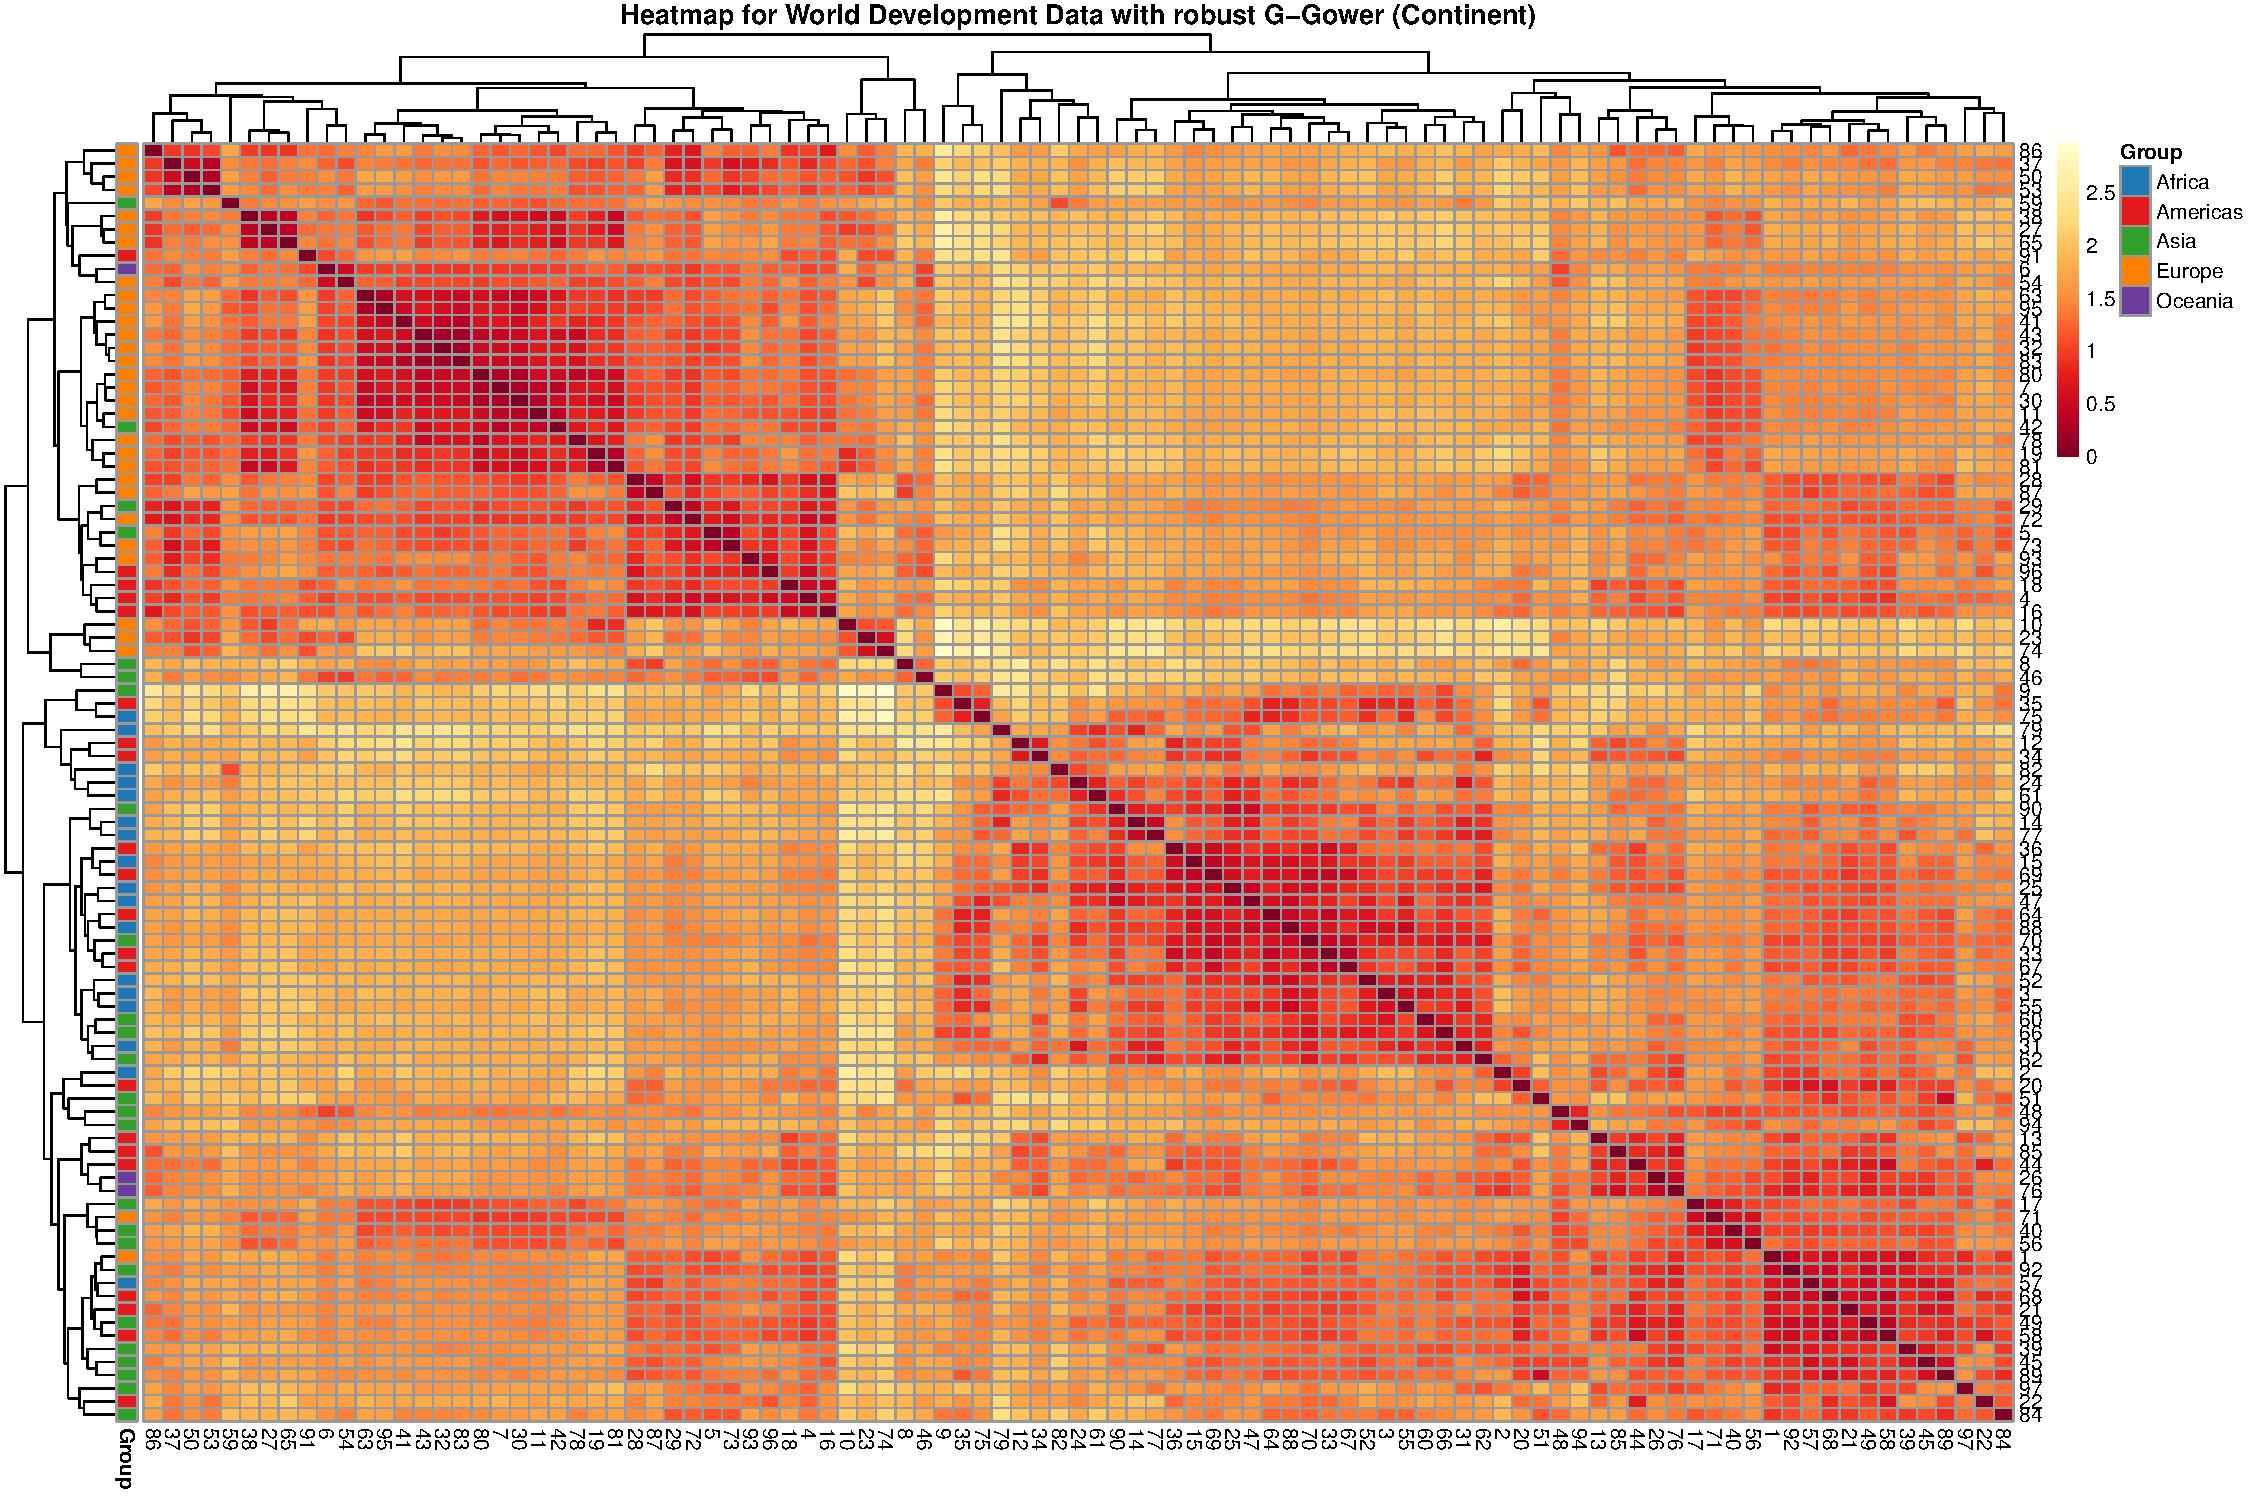
\includegraphics[
        width=0.8\linewidth,
        trim={0cm 0cm 0cm 0.5cm}, % left bottom right top
        clip
    ]{imagenes/HeatmapWDDGGowerBig.pdf}
    \caption{Heatmap representation for robust G-Gower pairwise distances. World Development Indicators.}
    \label{fig:heatmap.ggower}
\end{figure}

To illustrate the performance of the three distances, we present a comparative study whose main goal is to assess the behavior of the classical and robust approaches under realistic socioeconomic data conditions, where heterogeneity across countries and potential data irregularities (e.g., extreme values or nonlinear dependencies) may distort the analysis.

To further illustrate these aspects, Figure~\ref{fig:mds_worlddata} presents the multiple MDS plots with the classical MDS configurations obtained from the three distance matrices, with variable \texttt{Pov} (Poverty) as the conditioning factor.

\begin{figure}[!htbp]
\centering
    \begin{subfigure}{0.32\textwidth}
        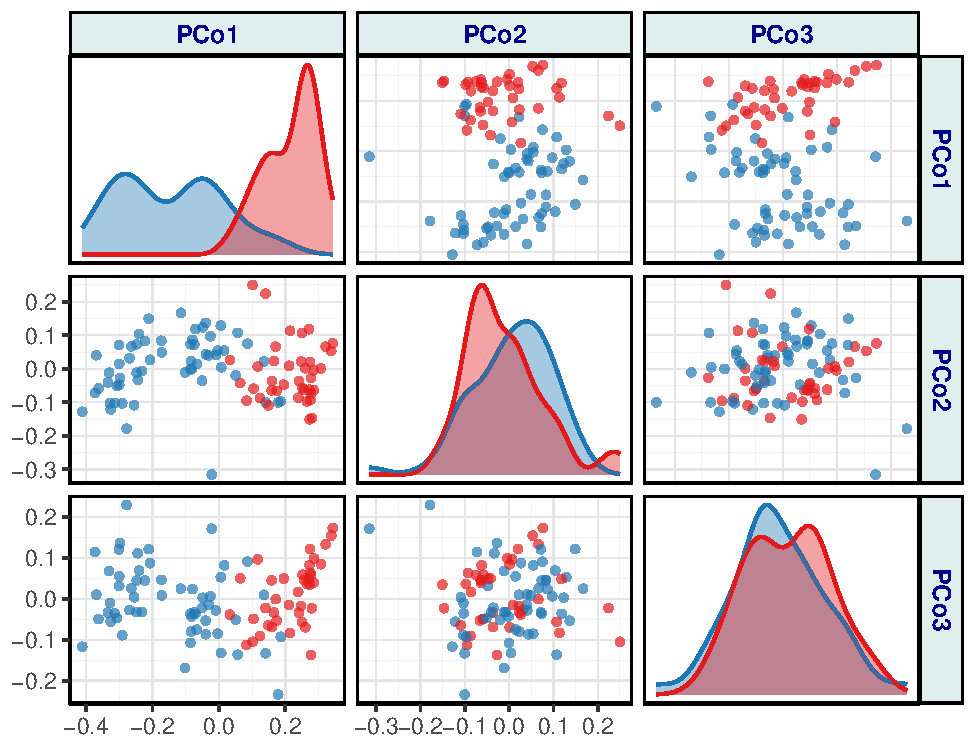
\includegraphics[width=\linewidth]{imagenes/MDSWDDGowerPov.pdf}
        \caption{Gower}
        \label{fig:mds_gower}
    \end{subfigure}
    \begin{subfigure}{0.32\textwidth}
        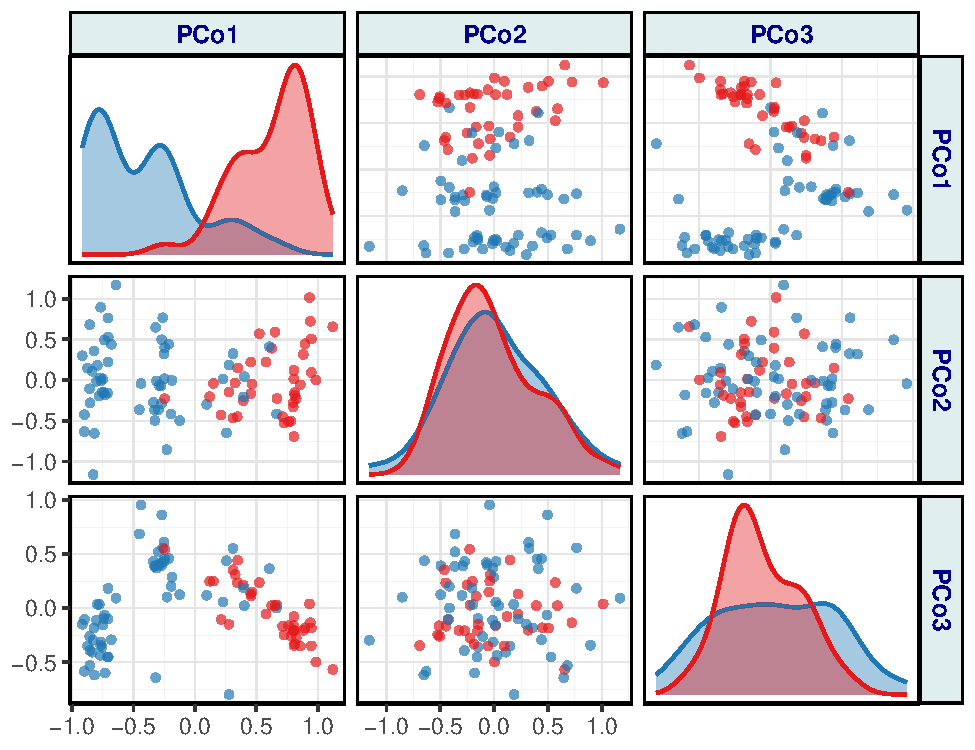
\includegraphics[width=\linewidth]{imagenes/MDSWDDGGowerPov.pdf}
        \caption{G-Gower}
        \label{fig:mds_ggower}
    \end{subfigure}
    \begin{subfigure}{0.32\textwidth}
        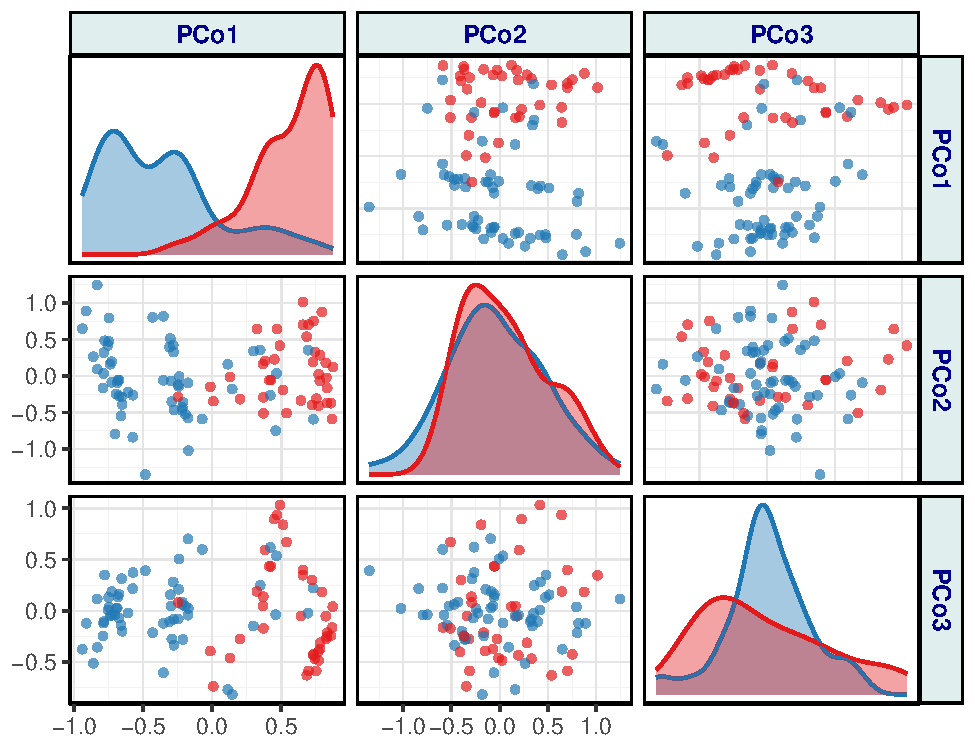
\includegraphics[width=\linewidth]{imagenes/MDSWDDRelMSPov.pdf}
        \caption{RelMS}
        \label{fig:mds_relms}
    \end{subfigure}

\caption{Multiple MDS configurations for the World Development Indicators dataset under three distance measures. Each panel displays the two-dimensional projection of 97 countries, colored by poverty level (\texttt{Pov}; Blue = High poverty level, Red = Low poverty level).}
\label{fig:mds_worlddata}
\end{figure}

The MDS configurations in Figure~\ref{fig:mds_worlddata} display the spatial arrangement of countries according to their socioeconomic similarity, grouped by poverty level (\texttt{Pov}). Under the classical Gower distance (a), two well-defined clusters emerge, corresponding to the high- and low-poverty groups, with only a few countries lying in intermediate positions. The same general structure is preserved under the robust G-Gower and RelMS distances (b)–(c), indicating that the dataset exhibits low-contamination conditions.

To gain further insight into the global development patterns, Figure~\ref{fig:mds_worlddata_continent} displays the multiple MDS plots with the classical MDS configurations obtained from the three distance matrices, using the variable \texttt{Con} (Continent) as the conditioning factor. Coloring the countries by continent allows us to assess whether geographic or regional factors are reflected in the latent similarity structure captured by each distance measure.

\begin{figure}[!htbp]
\centering
    \begin{subfigure}{0.32\textwidth}
        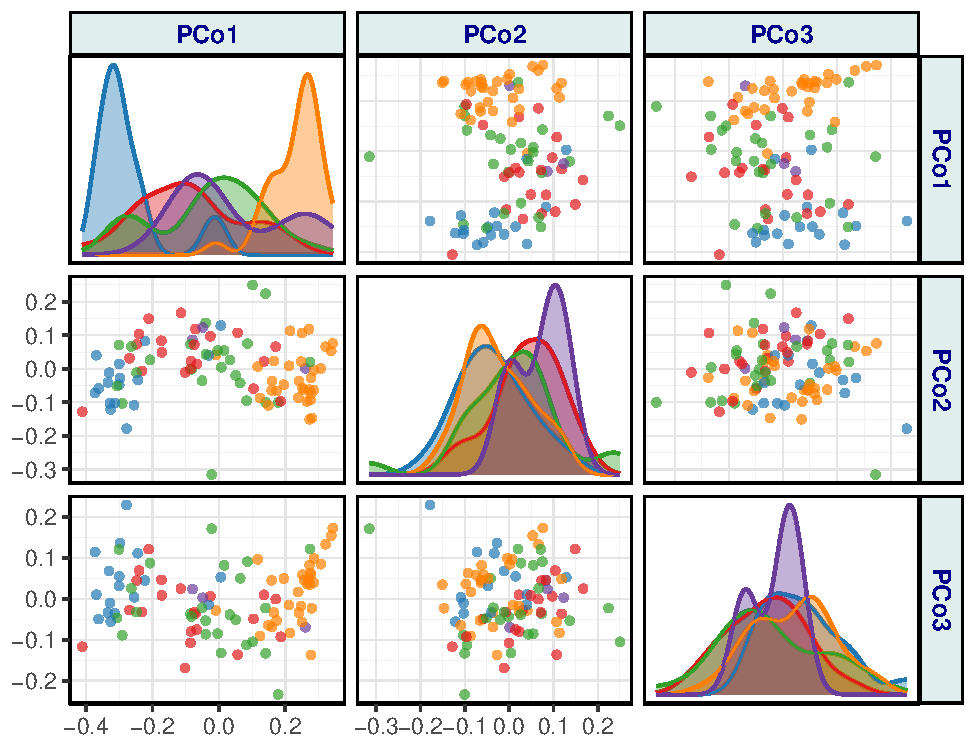
\includegraphics[width=\linewidth]{imagenes/MDSWDDGowerCon.pdf}
        \caption{Gower}
        \label{fig:mds_gower_con}
    \end{subfigure}
    \begin{subfigure}{0.32\textwidth}
        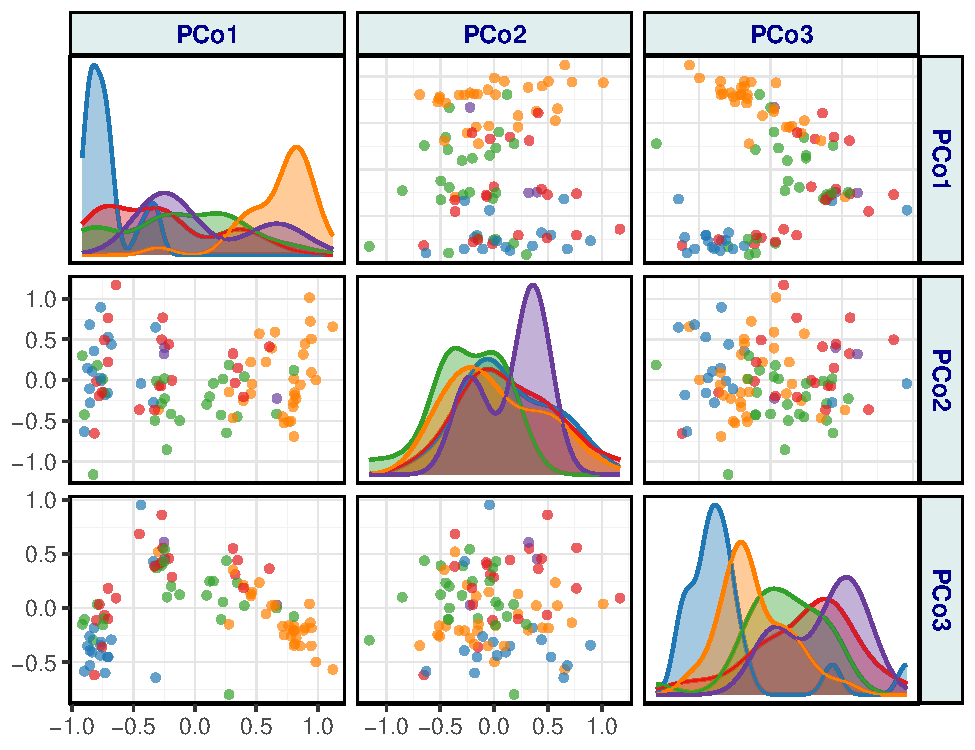
\includegraphics[width=\linewidth]{imagenes/MDSWDDGGowerCon.pdf}
        \caption{G-Gower}
        \label{fig:mds_ggower_con}
    \end{subfigure}
    \begin{subfigure}{0.32\textwidth}
        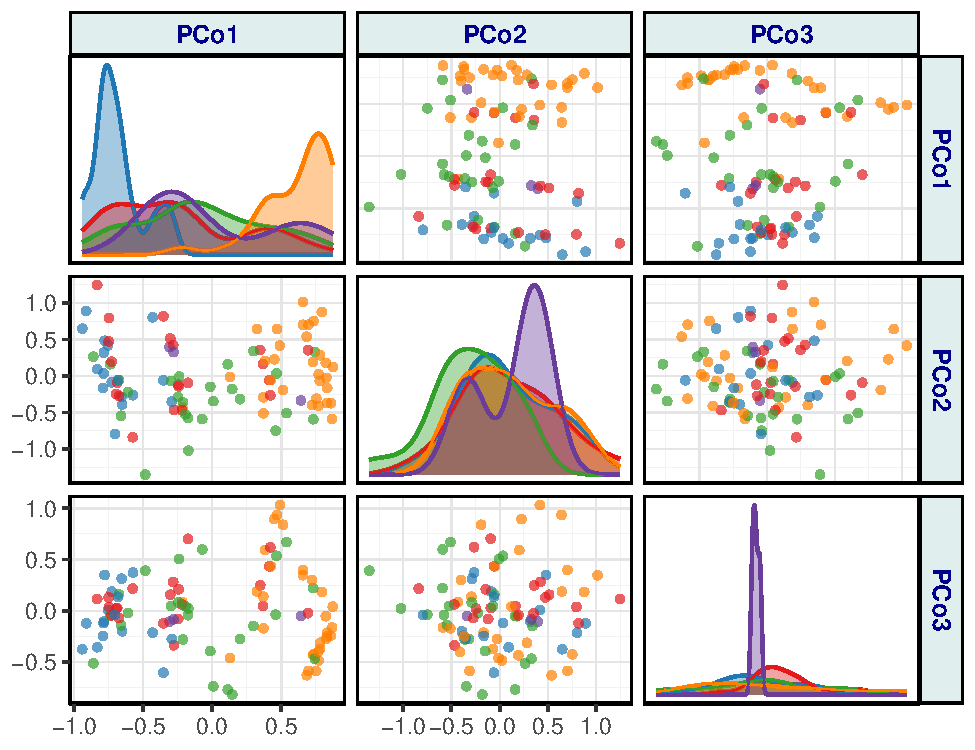
\includegraphics[width=\linewidth]{imagenes/MDSWDDRelMSCon.pdf}
        \caption{RelMS}
        \label{fig:mds_relms_con}
    \end{subfigure}

\caption{Multiple MDS configurations for the World Development Indicators dataset under three distance measures. Each panel displays the two-dimensional projection of 97 countries, colored by continent (\texttt{Con}; Blue = Africa, Red = America, Green = Asia, Orange = Europe, Purple = Oceania).}
\label{fig:mds_worlddata_continent}
\end{figure}

The MDS configurations in Figure~\ref{fig:mds_worlddata_continent} reveal a clear regional structure in the World Development Indicators dataset. Under the classical Gower distance (a), European and American countries form compact clusters, whereas African and Asian nations appear more dispersed, suggesting greater internal heterogeneity in their socioeconomic indicators. When the robust G-Gower and RelMS distances are applied (b)-(c), the global configuration becomes smoother and less dominated by extreme countries. The robust methods attenuate the influence of highly unbalanced indicators such as homicide rate or access to electricity, allowing a more balanced representation of intercontinental relationships. For example, countries from Asia and the Americas overlap more consistently, reflecting intermediate development profiles, while African countries remain more distinct but less isolated than in the classical solution.

To complement the MDS representations, Figure~\ref{fig:qgraph_worlddata_pov} displays the network structures derived from the three distance matrices using the \texttt{"qgraph"} visualization method, with countries grouped by their poverty level (\texttt{Pov}). In these networks, edges represent the strongest inter-country similarities, while node proximity and color reflect the degree of connectedness within and across poverty groups.

\begin{figure}[!htbp]
\centering
    \begin{subfigure}{0.32\textwidth}
        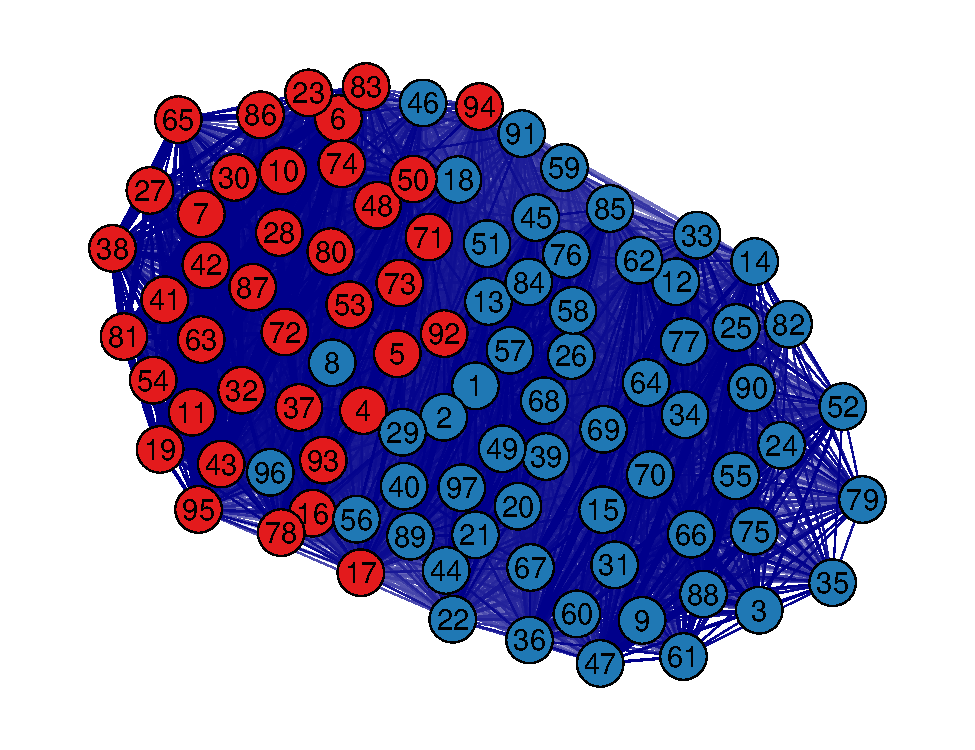
\includegraphics[width=\linewidth]{imagenes/QgraphWDDGowerPov.pdf}
        \caption{Gower}
        \label{fig:qgraph_gower_pov}
    \end{subfigure}
    \begin{subfigure}{0.32\textwidth}
        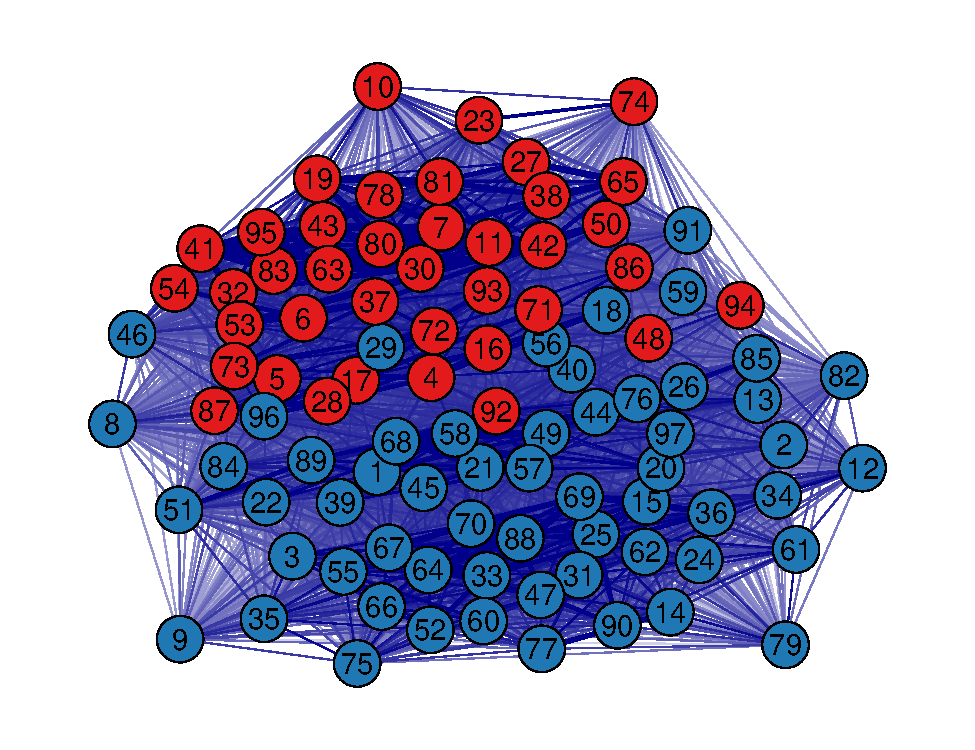
\includegraphics[width=\linewidth]{imagenes/QgraphWDDGGowerPov.pdf}
        \caption{G-Gower}
        \label{fig:qgraph_ggower_pov}
    \end{subfigure}
    \begin{subfigure}{0.32\textwidth}
        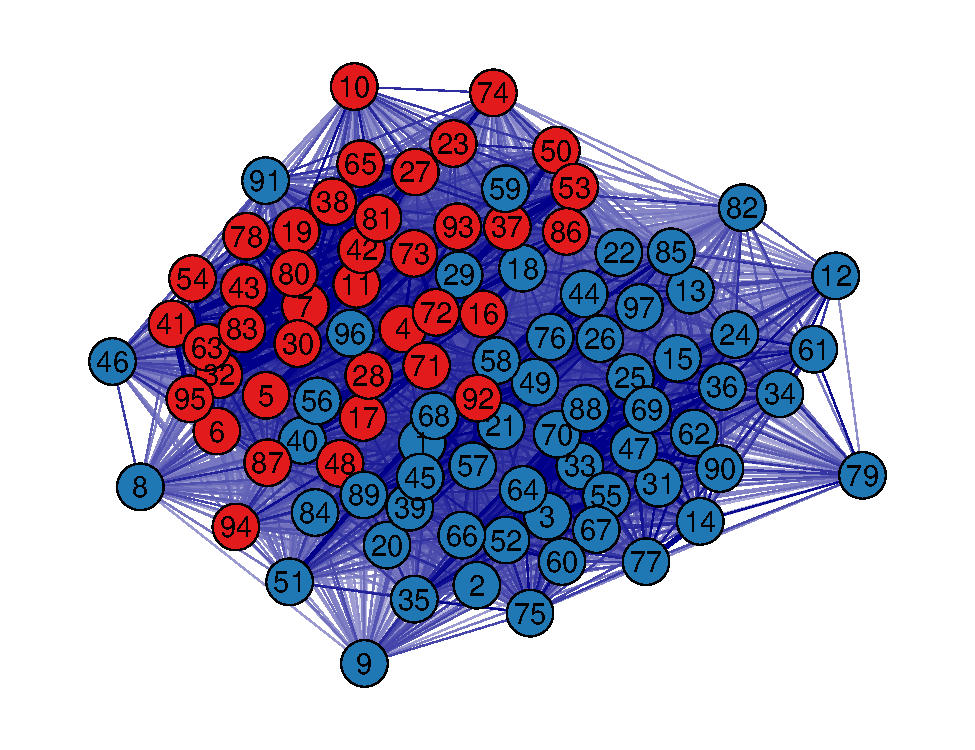
\includegraphics[width=\linewidth]{imagenes/QgraphWDDRelMSPov.pdf}
        \caption{RelMS}
        \label{fig:qgraph_relms_pov}
    \end{subfigure}

\caption{Network visualizations (\texttt{qgraph}) of the World Development Indicators dataset under three distance measures, with nodes colored by poverty level (\texttt{Pov}; Blue = High poverty level, Red = Low poverty level).}
\label{fig:qgraph_worlddata_pov}
\end{figure}

In the network representations of Figure~\ref{fig:qgraph_worlddata_pov}, countries are grouped by poverty level. The classical Gower graph (a) displays two well-established clusters with a few overlapped observations, the same for G-Gower (b) and RelMS (c) demonstrating that the data present low-contamination conditions. When contamination is absent, robust methods perform comparably to classical ones.

Similarly, Figure~\ref{fig:qgraph_worlddata_con} presents the \texttt{"qgraph"} representations for the same three distance measures, this time grouping countries by continent (\texttt{Con}). These network structures highlight regional cohesion and cross-continental linkages based on socioeconomic similarity.

\begin{figure}[!htbp]
\centering
    \begin{subfigure}{0.32\textwidth}
        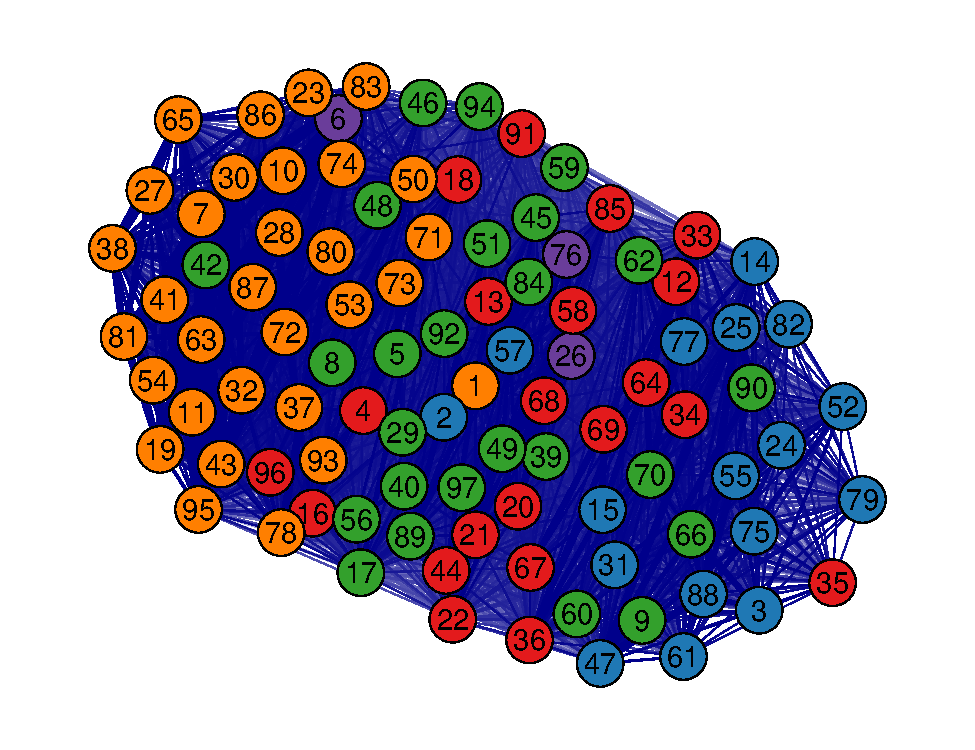
\includegraphics[width=\linewidth]{imagenes/QgraphWDDGowerCon.pdf}
        \caption{Gower}
        \label{fig:qgraph_gower_con}
    \end{subfigure}
    \begin{subfigure}{0.32\textwidth}
        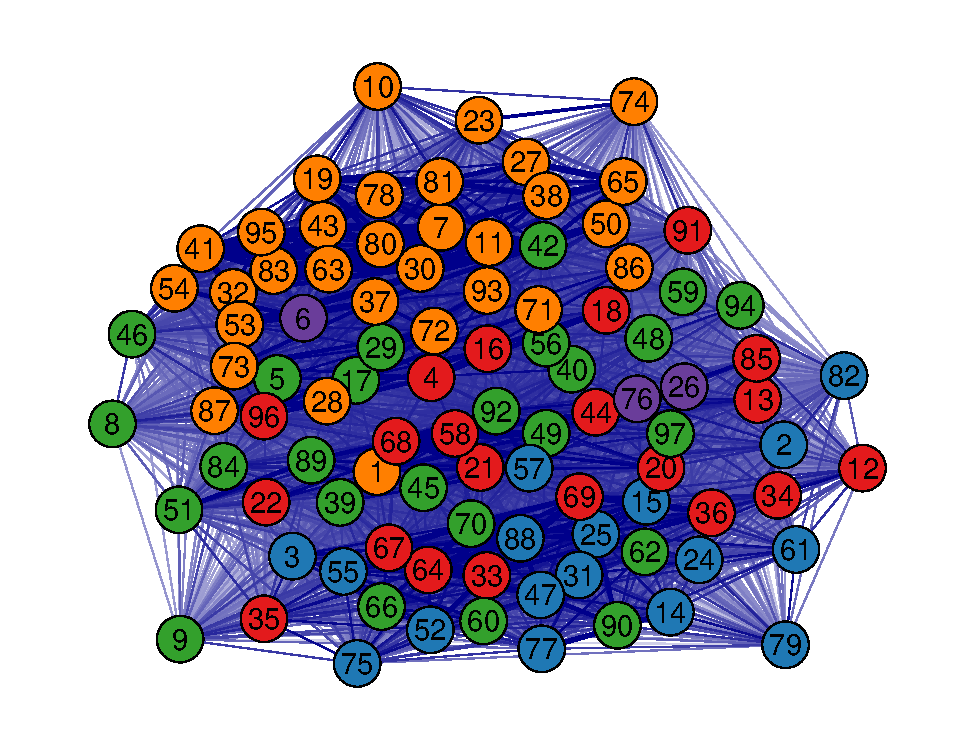
\includegraphics[width=\linewidth]{imagenes/QgraphWDDGGowerCon.pdf}
        \caption{G-Gower}
        \label{fig:qgraph_ggower_con}
    \end{subfigure}
    \begin{subfigure}{0.32\textwidth}
        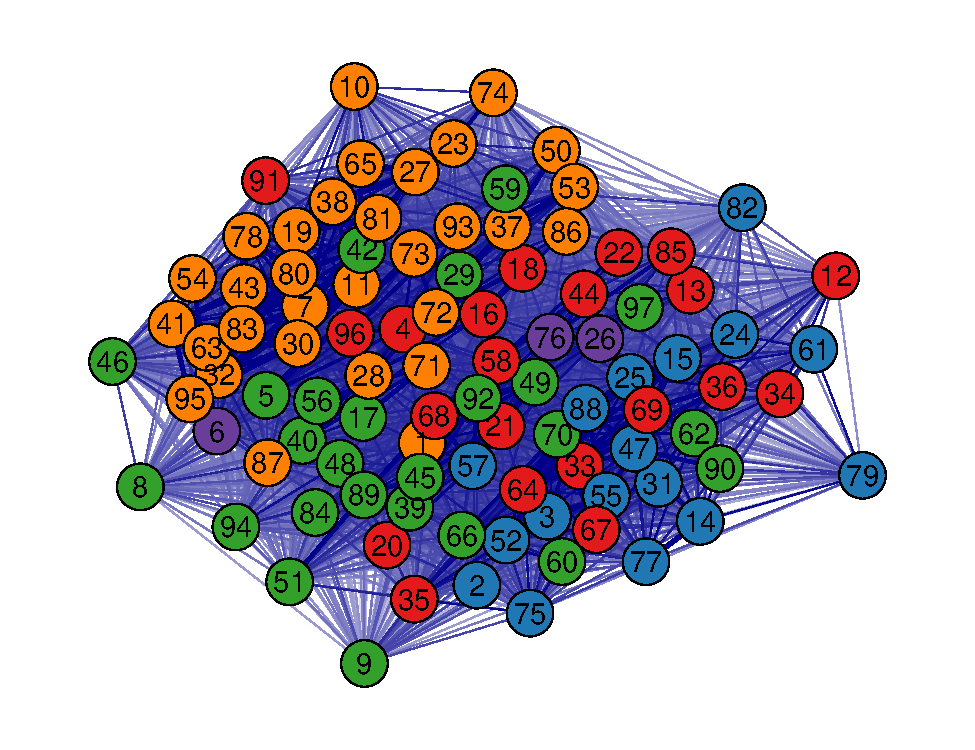
\includegraphics[width=\linewidth]{imagenes/QgraphWDDRelMSCon.pdf}
        \caption{RelMS}
        \label{fig:qgraph_relms_con}
    \end{subfigure}

\caption{Network visualizations (\texttt{qgraph}) of the World Development Indicators dataset under three distance measures, with nodes colored by continent (\texttt{Con}; Blue = Africa, Red = America, Green = Asia, Orange = Europe, Purple = Oceania).}
\label{fig:qgraph_worlddata_con}
\end{figure}

The network visualizations in Figure~\ref{fig:qgraph_worlddata_con} show that the three distance measures produce very similar connectivity patterns. In all cases Europe appears as a relatively compact and well-defined cluster, indicating homogeneous socioeconomic profiles among European countries in the dataset. The other continents (Africa, Asia and the Americas) display greater internal variability and, in some areas, partially overlapping connections; this overlapping is present across the Gower, G-Gower and RelMS graphs and is not visibly reduced by the robust alternatives. In short, the robust distances do not produce a markedly different network topology here, a finding consistent with a dataset that lacks strong influential outliers: when contamination is absent or weak, robustification yields configurations comparable to the classical measure rather than “improvements” in network structure.

Overall, the empirical results obtained in this application indicate that the robust distance measures, G-Gower and RelMS, do not outperform the classical Gower distance in either the MDS or network representations. This outcome is conceptually consistent with the theoretical rationale of robust methods: their purpose is not to enhance performance under regular data conditions, but to ensure stability and resilience in the presence of contamination, extreme observations, or structural imbalance. In this dataset, characterized by moderate variability and limited influence of atypical cases, the classical and robust approaches converge toward similar configurations. Rather than aiming to highlight the superiority of robust measures, this application was intended to demonstrate the practical implementation and versatility of the \texttt{dbrobust} package, illustrating how it can be applied to complex, real-world socioeconomic data.

\section{Conclusion}
\label{sec.conclusions}

This work introduces \CRANpkg{dbrobust}, a comprehensive R package designed to address the methodological and practical challenges of robust DB analysis in datasets of mixed-type. Through a unified framework, the package enables the computation and visualization of classical and robust distances across mixed variable types, offering tools that are both accessible and extensible for applied researchers.

%The proposed methodology demonstrates clear advantages in handling data contamination, preserving structural patterns, and enhancing interpretability in high-dimensional settings. 
The proposed methodology demonstrates advantages in handling data contamination, preserving structural patterns, and enhancing interpretability.
By integrating novel robust formulations and advanced visualization techniques, \CRANpkg{dbrobust} facilitates exploratory and confirmatory analyses that are resilient to outliers and adaptable to diverse research contexts. In the current framework, robustness is primarily introduced through the continuous component of the mixed-data dissimilarities, whereas binary and categorical variables are handled through classical similarity and dissimilarity measures. Importantly, the package bridges the gap between theoretical innovation and practical implementation, supporting seamless interoperability with existing R tools and workflows. Its utility is particularly relevant in fields such as social sciences, quality of life research, and gender inequality studies, where weighted complex data structures and robustness requirements are common.

The development of \CRANpkg{dbrobust} represents a significant contribution to the statistical ecosystem, empowering analysts to extract meaningful insights from complex, real-world datasets through robust and interpretable DB methods. Future research may extend the current framework by incorporating robust alternatives for binary and categorical variables, further broadening the scope of robust mixed-data analysis. Its seamless compatibility with the \CRANpkg{dbstats} package for DB regression modeling, as well as with other widely used R packages that rely on distance inputs, such as those for clustering and classification, ensures its integration into existing analytical workflows and reinforces its practical value for applied research.

\section*{CRediT authorship contribution statement}

{\bf Marcos Álvarez:} Software, Writing -- Original draft preparation, Investigation.  
{\bf Eva Boj:} Conceptualization, Methodology, Software, Writing -- Original draft preparation, Reviewing and Editing, Investigation, Supervision.  
{\bf Aurea Grané:} Conceptualization, Methodology, Software, Writing -- Original draft preparation, Reviewing and Editing, Investigation, Supervision. 

\section*{Funding}

The authors gratefully acknowledge the support of grants PID2021-123592OB-I00 and TED2021-129316B-I00 funded by MCIN/AEI/10.13039/501100011033 and by ``ERDF A way of making Europe'' and ``European Union NextGenerationEU/PRTR''.

\bibliography{RJBoj_Grane_Alvarez}

\address{Eva Boj\\
  Department of Economic, Financial and Actuarial Mathematics\\
	Universitat de Barcelona\\
  Avinguda Diagonal 690, 08034 Barcelona\\
  Spain\\
	ORCID: 0000-0002-9487-0693\\
  \email{evaboj@ub.edu}}

\address{Aurea Grané\\
  Statistics Department\\
  Universidad Carlos III de Madrid\\
  Calle Madrid 126, 28903 Getafe\\
  Spain\\
	ORCID: 0000-0003-0980-6409\\
  \email{aurea.grane@uc3m.es}}

\address{Marcos \'Alvarez\\
	Statistics Department\\
  Universidad Carlos III de Madrid\\
  Calle Madrid 126, 28903 Getafe\\
  Spain\\
	ORCID: 0009-0006-6192-0152\\
  \email{marcoalv@pa.uc3m.es}}

\newpage
\appendix
\noindent
{\large\textbf{Appendix: Internal and logical modular structure of functions in dbrobust}}
%\section{Internal and Logical Modular Structure of Functions in dbrobust}
%\label{App}

\section{Internal and logical modular structure of function for computing dissimilarities and similarities}
\label{AppCalculateDistances}

The \texttt{calculate\_distances} function is designed following a modular architecture, which delegates specific tasks to helper functions depending on the data type and distance method. Table~\ref{tab:modular-structure} summarizes each internal component and its role.

\begin{table}[h!]
\caption{Modular structure of function for computing dissimilarities and similarities.\label{tab:modular-structure}}
\begin{center}
{\footnotesize
\begin{tabular}{|p{3cm}p{10.7cm}|}
\hline
\textbf{Function} & \textbf{Description} \\
\hline
\texttt{calculate\_distances} & Main entry point and wrapper function. Validates arguments, selects method category, delegates computation to specialized helper functions, and formats values. \\
\hline
\texttt{distBinary} & Computes pairwise distances for binary data using standard measures such as Jaccard, Dice, and Sokal-Michener. Uses \CRANpkg{ade4} where appropriate. \\
\hline
\texttt{distCategorical} & Computes distances for categorical variables using the matching coefficient (proportion of attribute matches) or the Cramér-based distance which accounts for the pair-wise association between variables. \\
\hline
\texttt{distContinuous} & Handles numerical data using measures such as Euclidean, Minkowski, Mahalanobis, Cosine, and Correlation. Uses base R and \CRANpkg{proxy} where appropriate. \\
\hline
\texttt{distMixed} & Implements Gower's distance for mixed-type data. Continuous variables are scaled by range; binary variables can be treated as symmetric or asymmetric (controlled by \texttt{binaryAsym}; only 1/1 counts as a match); categorical variables are compared by exact match. Users can optionally specify which columns are continuous, binary, or categorical using the arguments \texttt{continuousCols}, \texttt{binaryCols}, and \texttt{categoricalCols}. Similarities are converted to distances ($d = 1 - s$), yielding a symmetric matrix in [0,1]. \\
\hline
\texttt{formatOutput} & Converts distance matrix into the desired value format: \texttt{dist}, full matrix, or similarity matrix using selected transformation. \\
\hline
\texttt{convertToDist} & Utility function to coerce similarity matrices into \texttt{dist} objects. Supports linear and square-root transformations. \\
\hline
\end{tabular}}
\end{center}
\end{table}

Modularizing the \texttt{calculate\_distances()} function is crucial for maintaining clarity, flexibility, and ease of maintenance. By breaking down the computation into specialized helper functions based on data type and distance measure, the function becomes more organized and easier to extend or debug. This approach also promotes code reuse and separation of concerns, allowing each component to focus on a specific task. Furthermore, leveraging established external libraries such as \CRANpkg{proxy} or \CRANpkg{ade4} whenever possible ensures efficient implementations of complex distance calculations, reduces development time, and benefits from community-tested and optimized algorithms, ultimately enhancing the reliability and performance of the values returned by the function.

The function \texttt{calculate\_distances()} might be intricate and modular, yet its logic can be broken down into a series of conceptual steps, which are outlined in Table~\ref{tab:modular-structure-calculate-distances}.

\begin{table}
\caption{Internal logical structure of function for computing dissimilarities and similarities and helper functions}
\label{tab:modular-structure-calculate-distances}
\begin{center}
{\footnotesize
\begin{tabular}{|p{3.5cm}p{10.2cm}|}
\hline
\textbf{Step} & \textbf{Description} \\
\hline
Argument validation & Check \texttt{x} type, \texttt{outputFormat}, and \texttt{p} for Minkowski. \\
\hline
Normalize method & Standardize method string (lowercase, underscores). \\
\hline
Select distance function & Choose appropriate function based on method category (binary, categorical, continuous, mixed). This acts as a wrapper for the specialized routines. \\
\hline
Compute distances & Call \texttt{distBinary}, \texttt{distCategorical}, \texttt{distContinuous}, or \texttt{distMixed}. \\
\hline
Optional transformations & Square distances if requested; convert to similarity using linear or sqrt transformation. \\
\hline
Return values & Return values as \texttt{dist} object, numeric matrix, or similarity matrix. \\
\hline
\end{tabular}}
\end{center}
\end{table}

\section{Internal and logical modular structure of function for ensuring the Euclideanarity of matrices of pairwise squared distances}
\label{AppMakeEuclidean}

While \texttt{make\_euclidean()} is implemented as a single function, its logic can be decomposed into conceptual steps, summarized in Table~\ref{tab:modular-structure-euclidean}.

\begin{table}[h!]
\caption{Internal logical structure of function for ensuring Euclideanarity of matrices of pairwise squared distances}
\label{tab:modular-structure-euclidean}
\begin{center}
{\footnotesize
\begin{tabular}{|p{3.5cm}p{10.2cm}|}
\hline
\textbf{Step} & \textbf{Description} \\
\hline
Argument validation & Ensure the matrix argument \texttt{D} is a square matrix, and the weight vector \texttt{w} has matching length. \\
\hline
Weight normalization & Normalize \texttt{w} to sum to 1. \\
\hline
Compute weighted Gram matrix & Apply centering matrix $\mathbf{J}_w$ to $\mathbf{D}$ to obtain $\mathbf{G}_w$. \\
\hline
Eigenvalue analysis & Extract eigenvalues of $\mathbf{G}_w$ and check smallest value against \texttt{tol}. \\
\hline
Correction step & If $\lambda_{\min} < -$\verb+tol+, %shift $\mathbf{D}$ by $2c$ off-diagonal, and $-2c$ on diagonal, with $c = |\lambda_{\min}|$. \\
shift $\mathbf{D}$ by $2\,|\lambda_{\min}|$ off-diagonal. \\
\hline
Recompute eigenvalues & Compute eigenvalues of corrected $\mathbf{G}_w$ to verify positive semi-definiteness. \\
\hline
Return values & Return a list containing the corrected $\mathbf{\Delta}$ matrix, eigenvalues before/after, and transformation flag. \\
\hline
\end{tabular}}
\end{center}
\end{table}

\section{Internal and logical modular structure of internal and logical modular structure of function for computing robust distances}
\label{AppRobustDistances}

\begin{table}[h!]
\caption{Internal logical structure of function for computing robust distances}
\label{tab:modular-structure-aggregate}
\label{ref:table8}
\begin{center}
{\footnotesize
\begin{tabular}{|p{3.5cm}|p{10.2cm}|}
\hline
\textbf{Step} & \textbf{Description} \\
\hline
Argument validation & Ensures that either \texttt{p} or all variable groups are provided, checks for missing variables, and forbids \texttt{NA} values in the selected columns. \\
\hline
Data preparation & Reorders variables, converts factors/characters to numeric codes, and assembles the data matrix in [cont, bin, cat] order. \\
\hline
Weight handling & Sets equal weights if \texttt{w} is \texttt{NULL}; otherwise, normalizes and validates the user-supplied weights argument. \\
\hline
Robust covariance estimation & If continuous variables are present and no covariance matrix is supplied by the user via the argument \texttt{robust\_cov}, a robust covariance estimator is computed according to the argument \texttt{cov\_method}. The option \texttt{"gv"} calls \texttt{robust\_covariance\_gv}, which estimates the covariance matrix using the geometric variability trimming approach controlled by the trimming proportion \texttt{alpha}. Alternatively, \texttt{"mcd"} calls \texttt{robust\_covariance\_mcd}, which computes a weighted Minimum Covariance Determinant (wMCD) estimator using an iterative C-step algorithm with multiple random initializations. Both estimators return the robust covariance matrix together with the corresponding diagnostic information (central observations, detected outliers, and trimming statistics). \\
\hline
Squared distance computation & Depending on \texttt{method}, calls either \texttt{robust\_ggower} or \texttt{robust\_RelMS} to combine distances from each variable type. \\
\hline
Attach diagnostics & If trimming was performed, attaches indices of central and outlier units, the $\phi$ proximity values, and trimming quantile \texttt{q} as attributes of the result. \\
\hline
Return values formatting & Returns either squared distances \texttt{D2} or converts to a \texttt{dist} object with \texttt{D2toDist} if \texttt{return\_dist = TRUE}. \\
\hline
\end{tabular}}
\end{center}
\end{table}

The \texttt{robust\_distances()} function is designed following a modular architecture as well as \texttt{calculate\_distances()}, which delegates specific tasks to helper functions depending on the robust distance construction method. Tables \ref{ref:table8}--\ref{tab:robust-functions} summarize each internal and modular component and its role.

\begin{table}[h!]
\caption{Modular structure of function for computing robust distances and helper functions}
\label{tab:robust-functions}
\begin{center}
{\footnotesize
\begin{tabular}{|p{3.5cm}|p{10.2cm}|}
\hline
\textbf{Function} & \textbf{Description} \\
\hline
\texttt{robust\_covariance\_gv} & Computes a robust covariance matrix for continuous variables using the weighted Mahalanobis distance approach summarized in Figure~\ref{fig:robust-mahalanobis-workflow} (see Section 3.
%\ref{sec.software})
Identifies central observations via a trimming procedure controlled by \texttt{alpha}, excluding outliers from the covariance estimation. Returns the covariance matrix, indices of central and outlier observations, the proximity measure ($\phi$), and the trimming threshold (\texttt{q}). \\
\hline
\texttt{robust\_covariance\_mcd} &
Computes a weighted Minimum Covariance Determinant (wMCD) estimator for the continuous variables. This estimator provides a highly robust covariance matrix by identifying a subset of observations with minimum covariance determinant, while allowing observation weights. The resulting covariance matrix can subsequently be used by both \texttt{robust\_ggower} and \texttt{robust\_RelMS}. \\
\hline
\texttt{robust\_ggower} & Computes a robust G-Gower distance for mixed data by replacing the normalized city-block distance for continuous variables with a robust Mahalanobis distance using trimming to mitigate outliers. Keeps classical definitions for binary and categorical variables and combines all three types by simple weighted summation. Purpose: robustify distances in presence of continuous outliers without altering the classical fusion scheme. \\
\hline
\texttt{robust\_RelMS} & Extends \texttt{robust\_ggower} by integrating continuous, binary, and categorical sources through RelMS. Uses double-centering and interaction terms to reduce redundancy across variable types. Employs robust covariance and trimming for continuous data as before. Purpose: provide a more structured, robust, and less redundant joint metric for multitype data. \\
\hline
\end{tabular}}
\end{center}
\end{table}

The robust aggregated distances computed by \texttt{robust\_distances()} provide a solid foundation for subsequent multivariate analyses in mixed-type data settings. These robust metrics can be seamlessly integrated, for instance, with the \CRANpkg{dbstats} package, enabling robust DB regression models. This compatibility arises from the fact that \texttt{robust\_distances()} can return its results either as \texttt{D2} objects or as \texttt{dist} objects, two of the accepted argument formats for functions such as \texttt{dblm} or \texttt{dbglm} in \CRANpkg{dbstats}.

\section{Internal and logical modular structure
of function for merging distances}
\label{AppMergeDistances}

The internal workflow of \texttt{merge\_distances()}, including argument validation, Euclidean correction, weighted aggregation, and consensus distance reconstruction, is summarized in Tables~\ref{tab:merge-logical-structure}--\ref{tab:merge-functions}. The modular design facilitates the integration of heterogeneous distance sources while ensuring computational consistency and preserving Euclidean properties throughout the merging process.

\begin{table}[h!]
\caption{Internal logical structure of function for merging distances}
\label{tab:merge-logical-structure}
\begin{center}
{\footnotesize
\begin{tabular}{|p{3.5cm}|p{10.2cm}|}
\hline
\textbf{Step} & \textbf{Description} \\
\hline

Argument validation &
Checks that at least two distance matrices are supplied, converts \texttt{dist} objects into matrices, verifies that all matrices are square with identical dimensions, and ensures that all distances are non-negative.
\\
\hline

Weight handling &
Validates and normalizes both the observation weights (\texttt{w}) and the matrix weights (\texttt{matrix\_weights}). When either argument is omitted, equal weights are assigned before normalization.
\\
\hline

Euclidean preprocessing &
Converts the input distance matrices into squared distances when necessary and applies \texttt{make\_euclidean()} to each matrix to guarantee Euclidean properties before fusion.
\\
\hline

Gram matrix extraction &
Computes the weighted Gram matrices and their square-root decompositions for each distance source using weighted double-centering.
\\
\hline

Source weighting &
Incorporates the user-defined matrix weights into both the Gram matrices and their square-root representations.
\\
\hline

Consensus Gram matrix construction &
Depending on the value of \texttt{RelMS}, either computes a direct weighted aggregation of the Gram matrices or subtracts cross-source interaction terms computed by \texttt{relms\_compute\_cross\_terms()} to reduce redundancy among sources.
\\
\hline

Distance reconstruction &
Reconstructs the consensus squared distance matrix from the joint Gram matrix and removes possible numerical negative values.
\\
\hline

Output formatting &
Applies a final Euclidean correction using \texttt{make\_euclidean()} and returns either the consensus squared distance matrix or a \texttt{dist} object according to the value of the argument \texttt{squared}.
\\
\hline

\end{tabular}}
\end{center}
\end{table}

\begin{table}[h!]
\caption{Modular structure of function for merging distances and helper functions}
\label{tab:merge-functions}
\begin{center}
{\footnotesize
\begin{tabular}{|p{3.5cm}|p{10.2cm}|}
\hline
\textbf{Function} & \textbf{Description} \\
\hline

\texttt{make\_euclidean} &
Transforms non-Euclidean distance matrices into Euclidean ones using the Lingoes correction, ensuring that all input and output distance matrices satisfy Euclidean properties.
\\
\hline

\texttt{relms\_compute\_cross\_terms} &
Computes the cross-interaction terms between weighted Gram matrix square roots using a C++ implementation based on \CRANpkg{RcppArmadillo}. These interaction terms are used by RelMS to reduce redundancy among multiple distance sources.
\\
\hline

\texttt{merge\_distances} &
Combines multiple distance matrices into a consensus distance matrix by either direct weighted aggregation or Related Metric Scaling (RelMS), returning the result either as a squared distance matrix or as a \texttt{dist} object.
\\
\hline

\end{tabular}}
\end{center}
\end{table}

The \texttt{merge\_distances()} function provides a flexible framework for integrating multiple distance matrices into a single consensus representation. By supporting both direct weighted aggregation and the Related Metric Scaling (RelMS) methodology, the function allows users to combine complementary sources of information while reducing redundancy among them when the RelMS option is selected. The resulting consensus distance matrix can be directly employed in subsequent visualization, clustering, multidimensional scaling, or distance-based statistical analyses available in \CRANpkg{dbrobust} and compatible packages such as \CRANpkg{dbstats}.

\section{Internal and logical modular structure of function for visualizing distances and similarities}
\label{AppVisualizeDistances}

The internal workflow of \texttt{visualize\_distances()}, including argument validation, method selection, data preparation, and execution of the plotting routines, is summarized in Tables~\ref{tab:viz-logical-structure}--\ref{tab:viz-functions}. From version \texttt{1.1.0}, the visualization framework has been extended to support user-defined group color schemes through the \texttt{group\_colors} argument. When no custom colors are provided, the internal helper function \texttt{get\_custom\_palette()} automatically generates a palette of visually distinct colors.

\begin{table}[h!]
\caption{Internal logical structure of function for visualizing distances and similarities}
\label{tab:viz-logical-structure}
\begin{center}
{\footnotesize
\begin{tabular}{|p{3.5cm}|p{10.2cm}|}
\hline
\textbf{Step} & \textbf{Description} \\
\hline
Argument validation & Checks that \texttt{dist\_mat} is square and symmetric, and validates the arguments \texttt{k}, \texttt{weights}, \texttt{group}, and the optional \texttt{group\_colors}. \\
\hline
Method selection & Matches the \texttt{method} argument and directs execution to the corresponding plotting routine. \\
\hline
Data preparation & Converts distance matrices to the appropriate format, applies weights if relevant, assigns group labels, and prepares either user-defined or automatically generated color schemes for visualization. \\
\hline
Visualization execution & Calls the internal plotting functions (\texttt{plot\_mds}, \texttt{plot\_heatmap}, and \texttt{plot\_qgraph}) according to the selected \texttt{method}.\\
\hline
Return values & Returns the corresponding plotting object or produces the graphical output, depending on the selected visualization method (\texttt{ggmatrix} for MDS, \texttt{pheatmap} for heatmaps, and direct plotting for \texttt{qgraph}). \\
\hline
\end{tabular}}
\end{center}
\end{table}

\begin{table}[h!]
\caption{Modular structure of function for visualizing distances and similarities and helper functions.\label{tab:viz-functions}}
\begin{center}
{\footnotesize
\begin{tabular}{|p{3.5cm}|p{10.2cm}|}
\hline
\textbf{Function} & \textbf{Description} \\
\hline
\texttt{visualize\_distances} & Main interface for visualizing distance matrices. Validates that the matrix is square, symmetric, and has zero diagonals. Handles optional arguments such as \texttt{k}, \texttt{weights}, \texttt{group}, \texttt{group\_colors}, and \texttt{main\_title}. Delegates plotting tasks to \texttt{plot\_mds}, \texttt{plot\_heatmap}, or \texttt{plot\_qgraph} according to the selected \texttt{method}. \\
\hline
\texttt{plot\_mds} & Performs classical (\texttt{cmdscale}) or weighted (\texttt{wcmdscale}) multidimensional scaling. Generates pairwise scatterplot matrices with density plots on the diagonal and supports group-based coloring to facilitate the interpretation of the projected observations. \\
\hline
\texttt{plot\_heatmap} & Plots a heatmap from a distance matrix, with hierarchical clustering and optional group annotations. Supports subsampling, color palette customization, and annotation colors for categorical group variables. \\
\hline
\texttt{plot\_qgraph} & Constructs a network graph from a distance matrix using \CRANpkg{qgraph}. Converts distances to similarities, applies edge thresholding, supports group coloring, and limits the number of displayed nodes. \\
\hline
\texttt{get\_custom\_palette} &
Generates a palette of visually distinct colors for group annotations. Returns a predefined set of colors or interpolates additional colors when more groups are present, providing the default color scheme whenever \texttt{group\_colors} is not specified. \\
\hline
\end{tabular}}
\end{center}
\end{table}

The \texttt{visualize\_distances()} function provides a unified interface for exploring distance matrices through complementary graphical representations. By combining multidimensional scaling, heatmaps, and network visualizations within a common workflow, it facilitates the interpretation of complex distance structures while allowing users to incorporate grouping information through customizable visual annotations.

\end{article}

\end{document}
